% Kapitel 2


% http://www.lr-coordination.eu/resources
% https://www.deeplee.de/?page_id=23
% http://www.qt21.eu/publications/
% https://www.dfki.de

\chapter{Linguistischer Aspekt} % Main chapter title

\label{K2} % Change X to a consecutive number; for referencing this chapter elsewhere, use \ref{K2}

%----------------------------------------------------------------

Dieses Kapitel wendet sich der computervermittelten Kommunikation sowie der Wissensrepräsentation in digitalen Räumen, genauer gesagt: in Chatsituationen, zu. Hierfür werden zunächst die grundlegenden Elemente der computervermittelten Kommunikation (folgender Abschnitt \ref{K2:sec:CMC}) aufgezeigt und damit einhergehend die Wesenszüge der Chatkommunikation dargestellt (Abschnitt \ref{K2:subsec:characteristika-chat}, S.\,\pageref{K2:subsec:characteristika-chat}). Es folgt ein Abriss geläufiger Analysemodelle von computervermittelter Kommunikation, bevor über eine Betrachtung des Textbegriffs im Chat die Brücke zur Wissensrepräsentation geschlagen wird. Mit Blick auf die in dieser Arbeit behandelte Sprache Katalanisch enthält dieses Kapitel ebenfalls eine Exkursion in die soziale, linguistische und digitale Lebenswelt der Sprache (Abschnitt \ref{K2:sec:Status-Sprache-DigRaum}, S.\,\pageref{K2:sec:Status-Sprache-DigRaum}).


%----------------------------------------------------------------
%
% Section CMC
%

\section{Computervermittelte Kommunikation}
\label{K2:sec:CMC}

%----------------------------------------------------------------

\begin{quote}\sloppy
    Unter Kommunikation verstehen wir die Informationsübertragung zwischen Menschen. Kommunikation kann mithilfe von Sprache, Mimik, Gestik oder durch Schrift stattfinden. Dabei werden verschiedene Kommunikationskanäle bedient: akustisch, optisch, über Individualmedien (z.\,B.\ Telefon oder Computer) oder Massenmedien (z.\,B.\ Fernsehen oder Internet). \citep[158]{trepte_medienpsychologie_2012}
\end{quote}

Dieses Zitat liefert in wenigen Zeilen eine grobe Definition von Kommunikation. Darauf soll im Folgenden aufgebaut werden. Um zusätzlich noch die Brücke zur sog. computervermittelten (\emph{computer-mediated}) Kommunikation (eng. \emph{CMC}, dt. \emph{CvK})\is{Kommunikation!computervermittelte} zu schlagen, erweitern \citeauthor{trepte_medienpsychologie_2012} die obige Aussage. Computervermittelte Kommunikation ist der \glqq zwischen zwei oder mehr Personen stattfindende, interaktive Prozess des Erstellens, Austauschens und Empfangens von Informationen mithilfe von Computern\grqq{} \citep[158]{trepte_medienpsychologie_2012}. Hierfür wurden über die Jahrzehnte mehrere Anwendungen\is{Chat!-anwendung} und Plattformen\is{Kommunikation!-splattform} entwickelt, die in der Forschung gleichermaßen betrachtet werden: Neben dem für diese Arbeit zentralen Chat (z.\,B.\ Internet Relay Chat, IRC\is{Internet Relay Chat}) sind dies E-Mail, Newsgroups bzw. Foren, Blogs, Videospiele, Videoplattformen, SMS, Internettelefonie uvm. Eine umfassende und differenzierte Aufzählung liefern beispielsweise \citep[beispielsweise][]{beck_computervermittelte_2006, misoch_online-kommunikation_2006}.

\begin{sloppypar}
Nun ist die Kommunikationswissenschaft ein ausgesprochen breites Forschungsfeld und zugleich stetigen Umwälzungen unterworfen, wie die Ausführungen verschiedener Autor{\textperiodcentered}innen aus unterschiedlichen Jahrzehnten belegen \citep[z.\,B.][]{doring_sozialpsychologie_2003, beiswenger_sprachhandlungskoordination_2007, durscheid_personale_2018, storrer_sprachliche_2001, beiswenger_eyetracking_2017, baechler_medienlinguistik_2016}. Beide eingangs genannten Zitate bedürfen daher einer eingehenden Situierung. Es ist zu bedenken, dass der Textchat\is{Chat!Text-} von Skype, also eine Form von textbasierter Kommunikation\is{Kommunikation!textbasierte}, im Mittelpunkt dieser Untersuchung steht. Die anderen, zumeist audio-visuellen, Formen (Voice- und Videochat)\is{Kommunikation!audio-visuelle}\is{Chat!Voice-}\is{Chat!Video-} werden deshalb nur angeschnitten. Mit dieser Abgrenzung wird ein grundlegendes Spannungsfeld bei der Betrachtung von (Chat- bzw. computervermittelter) Kommunikation aufgeworfen, das schon häufig Gegenstand von Studien war: die dichotomische Unterscheidung von Mündlichkeit und Schriftlichkeit\is{Mündlichkeit}\is{Schriftlichkeit}. An diesem Punkt setzen \citet[][13]{koch_gesprochene_2011} mit ihrem Modell an und bieten somit einen soliden Ausgangspunkt für die intendierte Kartographierung der CvK (s. \figref{K2:fig:modell-koch-oesterreicher}).
\end{sloppypar}

%------------------------------------------------------
% Koch-Oesterreicher-Modell

\begin{figure}
    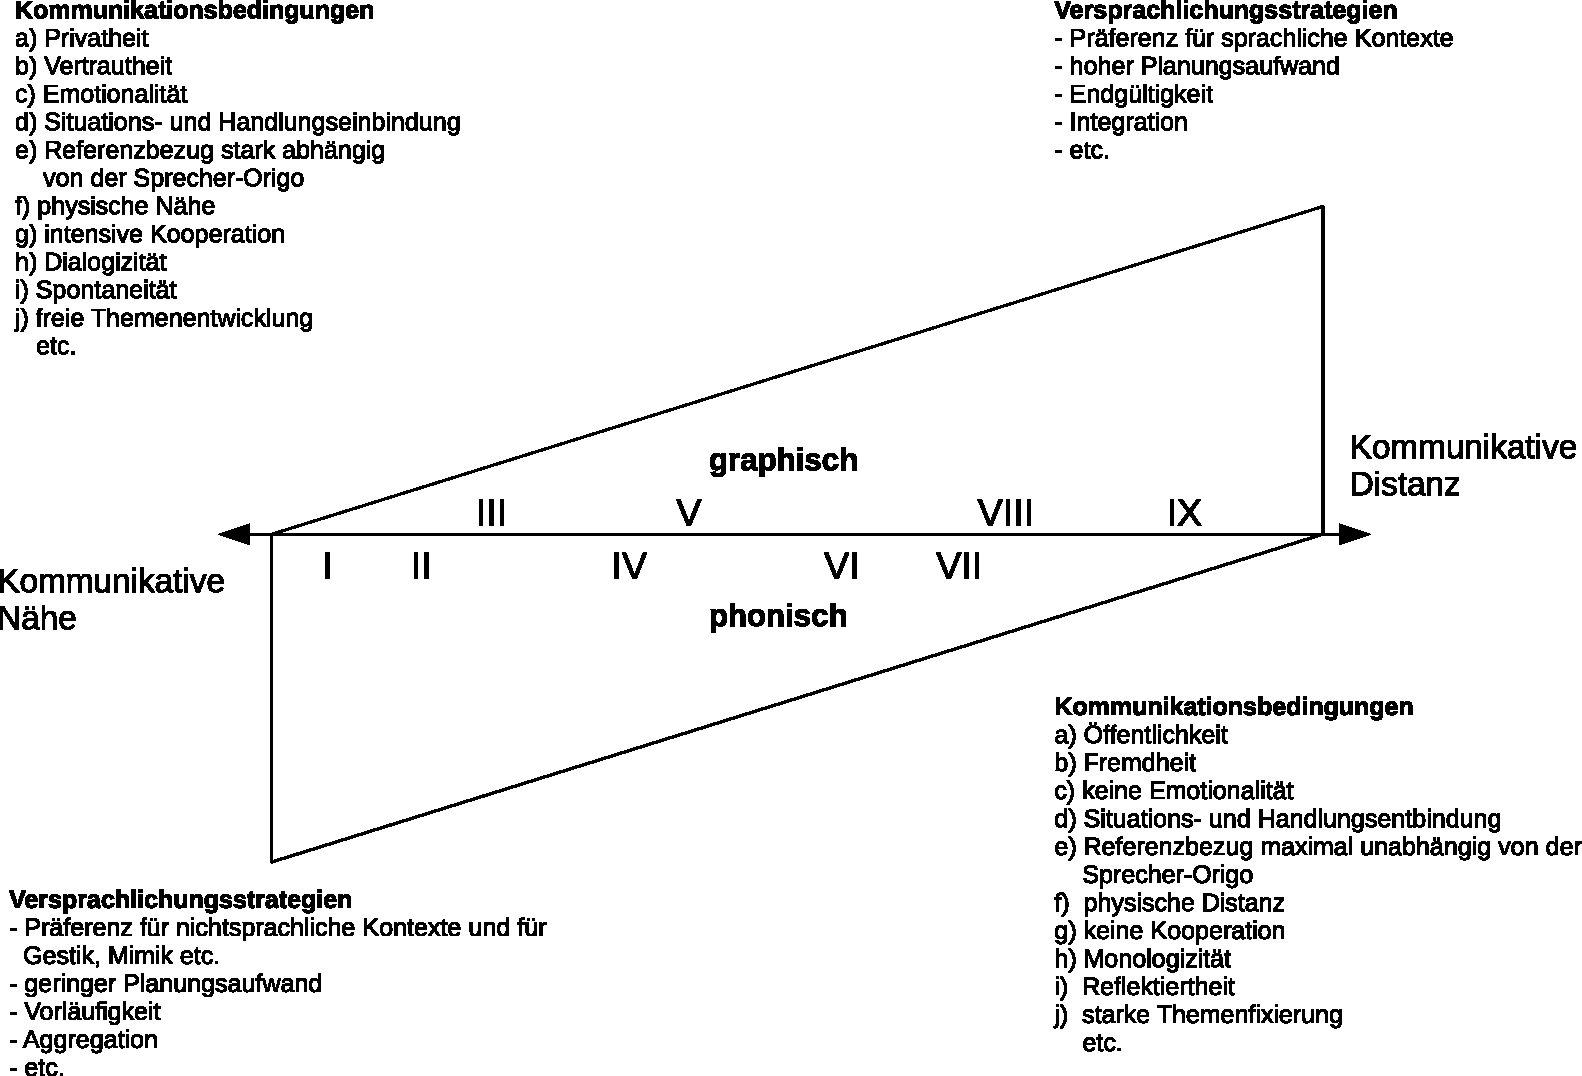
\includegraphics[width=\textwidth]{Figures/K2/modell-koch-oesterreicher.pdf}
	\caption[Das Modell von Koch und Oesterreicher]{Das Modell von Koch und Oesterreicher als von F.H. nachgebildete Darstellung\label{K2:fig:modell-koch-oesterreicher}}
\end{figure}

%------------------------------------------------------

Nähe- und Distanzkommunikation\is{Kommunikation!Nähe-}\is{Kommunikation!Distanz-} bilden im Modell die Pole eines Kontinuums, das sich entlang einer weiteren Achse in eine phonische und in eine graphische Dimension teilt. Die Bezeichnung als phonisch und graphisch ist auf eine terminologische Präzisierung zurückzuführen: \citeauthor{koch_schriftlichkeit_1994} weisen darauf hin, dass das Begriffspaar \emph{mündlich} und \emph{schriftlich} unterschiedlich verstanden werden kann. Einerseits sei damit das \glqq \emph{Medium} der Realisierung sprachlicher Äußerungen\grqq{} \citep[587, Kursivierung im Original]{koch_schriftlichkeit_1994} gemeint, weshalb hierfür von den Autoren fortan \emph{phonisch} für \emph{mündlich} und \emph{graphisch} für \emph{schriftlich} verwendet wird. Andererseits \glqq meinen die beiden Termini oft den Duktus, die Modalität der Äußerungen sowie die verwendeten Varietäten, kurz: die \emph{Konzeption}\grqq{} \citep[][587, Kursivierung im Original]{koch_schriftlichkeit_1994}. \citeauthor{koch_schriftlichkeit_1994} halten weiterhin fest, dass einerseits

\begin{quote}
zwischen dem phonischen Medium und konzeptionell mündlichen Äußerungsformen, andererseits zwischen dem graphischen Medium und konzeptionell schrftlichen Äußerungsformen eine ausgeprägte Affinität besteht. \citep[587]{koch_schriftlichkeit_1994}
\end{quote}

Die Eigenschaften der Pole können unter Kommunikationsbedingungen\is{Kommunikation!-sbedinungen} und Versprachlichungsstrategien\is{Versprachlichungsstrategien} subsummiert werden. Auf der Seite der Nähekommunikation\is{Kommunikation!Nähe-} stehen die Parameter Privatheit, Vertrautheit, Emotionalität, Si\-tu\-ati\-ons- und Handlungseinbindung, Referenzbezug abhängig vom Sprecher, physische Nähe\is{Kommunikation!Nähe-}, intensive Kooperation\is{Kooperation!intensive}, Dialogizität\is{Dialogizität}, Spontaneität\is{Kommunikation!spontane} und freie Themenentwicklung\is{Kommunikation!-sthema}. Die Sprache ist im Rahmen der Nähekommunikation nur ein Faktor \citep[591]{koch_schriftlichkeit_1994}. Dem entgegen stehen weitestgehend die Antonyme der genannten Begriffe als Parameter der kommunikativen Distanz\is{Kommunikation!Distanz-}: Öffentlichkeit, Fremdheit, keine Emotionalität, Situations- und Handlungsentbindung, Referenzbezug unabhängig vom Sprecher, physische Distanz, keine Kooperation, Monologizität, Reflektiertheit und starke Themenfixierung. In diesem Fall ist die Sprache nicht nur ein Faktor unter vielen. Als zentraler Bestandteil der Kommunikation erfährt das lexikalische Material eine Erweiterung, um auf außersprachliche Kontexte und Bezüge verweisen oder zugreifen zu können \citep[591]{koch_schriftlichkeit_1994}.

Mit Ausnahme von Referenzbezug und physischer Nähe\is{Kommunikation!Nähe-} bzw. Distanz handelt es sich um graduelle Parameter \citep[7]{koch_gesprochene_2011}. Weiterhin unterscheiden sich die Pole nach den Versprachlichungsstrategien\is{Versprachlichungsstrategien}. Auch diese Aspekte weisen eine graduelle Orientierung auf: (nicht-)sprachlicher Kontextbezug, Planungsaufwand, Vorläufigkeit bzw. Endgültigkeit sowie Integration bzw. Aggregation.

Das Modell beschreibt mit der Polarität von Nähe- und Distanzkommunikation\is{Kommunikation!Distanz-}\is{Kommunikation!Nähe-} einen Parameter, der so in dem Eingangszitat von \citeauthor{trepte_medienpsychologie_2012} zur CvK\is{Kommunikation!computervermittelte} keine -- allenfalls implizite -- Beachtung findet. Dabei ist dieser Aspekt allein schon von einem rein menschlichen-intuitiven Standpunkt aus sinnvoll: Einerseits erscheint es auf den ersten Blick wenig sinnvoll, mit einer Person im unmittelbaren, physischen Umfeld computergestützt zu kommunizieren. Andererseits gibt es durchaus Konstellationen, in denen diese Möglichkeit zur Kommunikation genutzt wird (bsp. Schüler{\textperiodcentered}innen, die im Unterricht heimlich miteinander kommunizieren).

Aus diesem denkbar knappen Umriss des Modells von \citeauthor{koch_gesprochene_2011} sollen nun im nachstehenden Abschnitt die wesentlichen Merkmale der Chatkommunikation aufgezeigt werden.

%------------------------------------------------------
%

\subsection{Charakteristika der Chatkommunikation}
\label{K2:subsec:characteristika-chat}
%------------------------------------------------------

\subsubsection{Definitiorische Grenzziehung}
Bevor sich den eigentlichen Charakteristika der Chatkommunikation\is{Kommunikation!Chat-}\is{Chat!-kommunikation} gewidmet wird, sei an dieser Stelle noch eine definitorische Grenze gezogen. Die folgenden Ausführungen beschreiben den Textchat\is{Chat!Text-} als durch eine entsprechende Anwendung ermöglichte Kommunikation zwischen mindestens zwei Personen. Diese Personen befinden meist an unterschiedlichen Orten, nutzen unterschiedliche Endgeräte und tauschen sich schriftlich über das Chatfenster der gewählten Anwendung\is{Chat!-anwendung} (sei es Skype, WhatsApp\is{WhatsApp}, Telegram\is{Telegram}, Facebook Messenger\is{Facebook!Messenger} uvm.) aus. Chats mit mehreren beteiligten Personen, die etwa \emph{Chat-Rooms}\is{Chat!-rooms} nutzen, werden in der Forschung seit mehreren Jahrzehnten untersucht \citep[vgl. z.\,B.][]{beiswenger_eyetracking_2017, schweiger_handbuch_2019}, an dieser Stelle kommt ihnen allerdings nur Beachtung im minimal nötigen Umfang zu. Der Skype Textchat sowie der Skype Translator\is{Skype!Skype Translator} können zwar auch in Konstellationen mit mehreren beteiligten Personen genutzt werden. Dies sei an dieser Stelle jedoch zu vernachlässigen. Es ist davon auszugehen, dass die Untersuchung des Skype Translators in Textchats mit mehr als zwei beteiligten Personen ganz andere Anforderungen an die theoretische Ausarbeitung sowie den Versuchsaufbau stellt. Daher empfiehlt sich für diese Betrachtung eine eigene Studie, zumal mit steigender Anzahl an beteiligten Personen auch der Grad der Interaktivität zunimmt. Die Interaktiviät wiederum ist ein eigener Forschungsbereich innerhalb der CvK\is{Kommunikation!computervermittelte} \citep[vgl. hierzu bsp.][]{beiswenger_eyetracking_2017, durscheid_personale_2018}.




\subsubsection{Nähekommunikation}\is{Kommunikation!Nähe-|(}
\begin{sloppypar}
Der textbasierten\is{Kommunikation!textbasierte} Chatkommunikation\is{Kommunikation!Chat-}\is{Chat!-kommunikation} werden in der Kommunikationsforschung Eigenschaften zugeschrieben, die im Sinne der Konzeption von \citeauthor{koch_gesprochene_2011} nur einem der beiden Pole zugeordnet werden können und sich somit auf den ersten Blick gegensätzlich gegenüberstehen. Den zentralen Punkt hebt \citet[446]{storrer_getippte_2001} hevor, die auf die konzeptionelle Mündlichkeit\is{Mündlichkeit} eines Textchats\is{Chat!Text-} verweist. Dieses Merkmal ist im Modell von \citeauthor{koch_gesprochene_2011} im Bereich des Nähe-Pols\is{Kommunikation!Nähe-} angesiedelt, da der Chat mehrere entsprechende Versprachlichungsstrategien\is{Versprachlichungsstrategien} und Kommunikationsbedingungen\is{Kommunikation!-sbedingungen} aufweist. Es kann also von einer Ähnlichkeit mit der Kommunikation von Angesicht zu Angesicht ausgegangen werden. \citet[35]{durscheid_neue_2016} folgt dieser Sicht nur bedingt, da sie die Chatkommunikation\is{Kommunikation!Chat-}\is{Chat!-kommunikation} eher in die Nähe zu einem Telefongespräch als zu einer direkten, unmittelbaren Kommunikation\is{Kommunikation!von Angesicht zu Angesicht} von Angesicht zu Angesicht rückt. Bei einem Telefonat\is{Kommunikation!Telefon} werde zwar räumliche Distanz offenkundig und die Kommunikation unterliege gewissen Einschränkungen, die Interaktion folge jedoch den Prinzipien der Mündlichkeit\is{Mündlichkeit}. So werde im Chat versucht, das Fehlen von para- und non-verbalen Kommunikationselementen (wie Gestik und Mimik) durch Emojis und andere Elemente auszugleichen \citep[3\psq]{storrer_sprachliche_2001}.

Orthographische Schwächen werden ebenfalls weitestgehend akzeptiert, was der Chatkommunikation\is{Kommunikation!Chat-}\is{Chat!-kommunikation} einen vorläufigen Charakter verleiht \citep[444\psq]{storrer_getippte_2001}. Der geringe Planungsaufwand tritt dadurch zutage, dass eine Person eine Information in mehrere kleinere Nachrichten zerlegt, die sie dann versendet \citep[287]{beiswenger_chattern_2010}. Allgemein weist die Chatkommunikation also eine unmittelbare Ausrichtung auf die jeweils gegenwärtige Situation auf. Daher kommt \citep[][5]{storrer_sprachliche_2001} als Zwischenfazit zu der Einschätzung, dass, wenn man zwischen den funktionalen Kategorien Text und Diskurs\is{Diskurs} (Gespräch) differenziert, (\dots) die im Chat produzierten Kommunikate eindeutig dem Gespräch zuzurechnen\grqq{} sind.\is{Kommunikation!Nähe-|)}
\end{sloppypar}

\subsubsection{Distanzkommunikation}\label{K2:para:Distanzkommunikation}\is{Kommunikation!Distanz-|(}
Zugleich wird der Chat jedoch auch als Interaktionsform angesehen, die es ermöglicht, \glqq über räumlich, zeitliche oder raumzeitliche Distanzen hinweg\grqq{} \citep[12]{beck_computervermittelte_2006} zu kommunizieren, da er verschriftlicht vorliegt und dadurch \glqq die Produktion und die Rezeption der Äußerungen (\dots) hier zeitlich entkoppelt\grqq{} \citep[][35]{durscheid_personale_2018}. Diese Gründe rücken den Chat in den Bereich der Distanzkommunikation. Auf diese Eigenschaft wird in der Forschung ebenfalls referiert, wenn es um die Beschreibung der Chatkommunikation\is{Kommunikation!Chat-} aus technologischer Sicht geht (s. in dieser Arbeit Abschnitt \ref{K2:subsec:medientheoretische-Internet-Kommunikation}, S.\,\pageref{K2:subsec:medientheoretische-Internet-Kommunikation}). \citeauthor{beiswenger_chattern_2010} konstruiert eine Verbindung zwischen diesen beiden Polen durch die ergebnisorientierte\is{Interaktion!ergebnisorientierte} Interaktion, die von allen Beteiligten erst dadurch als gemeinsames Produkt wahrgenommen wird, dass der Chat \glqq zur Prozessierung synchronen und dialogischen\is{Dialog} Austauschs die Überlieferungsqualitäten von Textformen nutzt\grqq{} \citep[249]{beiswenger_chattern_2010}. Wo im Gespräch von Angesicht zu Angesicht also zeitgleich kommuniziert werden kann, muss in der Chatkommunikation\is{Kommunikation!Chat-} die Schrift genutzt werden, damit über die zeitliche und räumliche Distanz alle Beteiligten die jeweiligen Chatbeiträge\is{Chat!-beitrag} als Dialog erfassen können \citep[249]{beiswenger_chattern_2010}. Zusammenfassend stellt \citeauthor{beiswenger_chattern_2010} hierzu fest: \glqq Während die Phonie irreversibel und flüchtig ist, ist die Graphie reversibel und persistent (\dots)\grqq{} \citep[249]{beiswenger_chattern_2010}.

Zugleich merkt \citeauthor{storrer_sprachliche_2001} auch an, dass der Chatverlauf\is{Chat!-verlauf}, also die Gesamtheit der getippten Beiträge, nicht dazu gedacht ist, mündlich vorgetragen zu werden.

\begin{quote}\sloppy
Die mündliche Reproduktion von Chatprotokollen\is{Chatprotokoll|see{Chatverlauf}} ist nicht intendiert. Mehr noch: Chat-Protokolle würden sich aufgrund ihrer sprachlichen Besonderheiten nur unter großen Schwierigkeiten mündlich vortragen lassen. \citep[4]{storrer_sprachliche_2001}
\end{quote}

\noindent Auch dieses Argument unterstreicht somit den Zwiespalt der Chatkommunikation\is{Kommunikation!Chat-} zwischen Nähe\is{Kommunikation!Nähe} und Distanz\is{Kommunikation!Distanz-|)}.



\subsubsection{Ablauf der Chatkommunikation}\label{K2:para:Ablauf}
Mehr noch erfordert die Chatkommunikation eine \glqq konsekutive Abfolge von Aktivitäten\grqq{} \citep[145]{beiswenger_eyetracking_2017}, die im Falle mündlicher Kommunikation zeitgleich erfolgen. Während die Prozesse des Verstehens, Verarbeitens und Produzierens von Gesprächsäußerungen gleichzeitig bei allen Beteiligten stattfinden, folgt eine gewöhnliche Chatkommunikation vielmehr dem hier dargestellten Schema: Zu Anfang steht bei einem oder einer der Chatbeteiligten die Entscheidung, einen Chatbeitrag\is{Chat!-beitrag} verfassen zu wollen. Da die meisten Chatanwendungen\is{Chat!-anwendung} nicht Zeichen für Zeichen der getippten Nachricht übermitteln, ist das explizite Senden (per Eingabetaste o.\,ä) erforderlich. Der Beitrag muss also weitestgehend vollständig schriftlich formuliert werden. Während dieser Zeit zeigen heutige Chatanwendungen der oder dem Gegenüber an, dass die andere Person gerade einen Beitrag verfasst (\emph{Person XY schreibt gerade\dots}). Die daraufhin abgesendete Nachricht wird in den meisten Fällen zunächst an einen Server geleitet, der sie dann chronologisch sortiert nach Zeitstempel dem Empfangsrechner zuführt. So ist nahezu ausgeschlossen, dass es zu einer Überlappung von Beiträgen kommt, wie es in der mündlichen Kommunikation der Fall sein kann \citep[7]{storrer_sprachliche_2001}. Die Übertragung dauert heutzutage nur wenige Millisekunden, selbst wenn zusätzliche Instanzen wie etwa der Skype Translator dazwischengeschaltet sind. Erst mit erfolgreicher Übermittlung kann dann die andere beteiligte Person die Nachricht erfassen und eine Reaktion hierauf bieten \citep[145\psq]{beiswenger_eyetracking_2017}. \citet[35\psq]{durscheid_neue_2016} erkennt hierin einen Vorteil gegenüber der Kommunikation von Angesicht zu Angesicht\is{Kommunikation!von Angesicht zu Angesicht}, da eine psychologische Hemmschwelle für die Chat-Teilnehmer{\textperiodcentered}innen wegfällt. Die Personen werden nicht beobachtet, während sie ihre Beiträge formulieren und können sich dank der schriftlichen Kommunikation auch bei Bedarf noch bis zum Versand der Nachricht korrigieren. Sogar über den Versand hinaus ist eine Korrektur des Chat-Beitrags möglich.

Dahingegen erfordert die Chat-Interaktion\is{Interaktion!Chat-}\is{Chat-!Interaktion} als solche die tatsächliche synchrone Präsenz der beteiligten Personen vor bzw. an ihren jeweiligen Endgeräten. Chatbeiträge\is{Chat!-beitrag} können zwar auch wie in einem (E-Mail-)Postfach für eine zeitverzögerte Erfassung zurückgehalten werden, verfehlen dann jedoch den Zweck der Chatkommunikation\is{Kommunikation!Chat-}\is{Chat-!kommunikation} im Sinne von \citet[30]{beiswenger_sprachhandlungskoordination_2007}, nämlich den dialogischen, dynamischen Austausch. Daher kommen \citet[]{storrer_sprachliche_2001}, \citet[]{beiswenger_sprachhandlungskoordination_2007} und \citet[]{schweiger_onlinekommunikation_2019} zu der Auffassung, es handele sich nicht um synchrone, sondern um quasi-synchrone Kommunikation\is{Kommunikation!quasi-synchrone}: Chat-Beiträge können erst dann erfasst werden, sobald sie vollends produziert und an alle beteiligten Personen übermittelt worden sind. Zur Präzisierung ist noch festzuhalten, dass \citet[23]{beiswenger_sprachhandlungskoordination_2007} \emph{synchron} und \emph{simultan} in eine hierarchische Beziehung zueinander setzt. \emph{Synchron} bezieht sich auf die \glqq zeitgleiche Verfügbarkeit von Kommunikanten für die Zwecke der Kommunikation\grqq{} \citep[23]{beiswenger_sprachhandlungskoordination_2007}, wohingegen \emph{simultan}\is{Kommunikation!simultane} als Hyponym dazu steht und zusätzlich noch das Erfassen der Chatbeiträge\is{Chat!-beitrag} während der Interaktion umschließt.

\begin{sloppypar}
Die Verbindung von Elementen der Nähe- und der Distanzkommunikation\is{Kommunikation!Distanz-}\is{Kommunikation!Nähe-} stellt deshalb besondere kognitive Anforderungen an die Beteiligten. Damit sich überhaupt erst eine zielgerichtete Interaktion\is{Interaktion} entwickeln kann, müssen die am Chat teilnehmenden Personen \glqq idealerweise permanent \emph{gleichzeitig produzieren und rezipieren}\grqq{} \citep[260, Hervorhebung im Original]{beiswenger_chattern_2010}, was jedoch unterschiedliche geistige Prozesse darstellt und somit \glqq bestenfalls kurzzeitig möglich ist\grqq{}.
\end{sloppypar}


%------------------------------------------------------
%

\subsection{Rollenverteilung in der Chatkommunikation}
\label{K2:subsec:turn-taking-chat}
%------------------------------------------------------

\is{Sprecher{\textperiodcentered}innenwechsel|(}
\is{Sprecher{\textperiodcentered}innenorganisation|(}
\is{Turn-Taking|(}
Aus den im vorausgehenden Abschnitt herausgearbeiteten Charakteristika der Chatkommunikation\is{Chat!-kommunikation}\is{Kommunikation!Chat-} ergeben sich auch Konsequenzen für die Organisation des Sprecher{\textperiodcentered}\linebreak[3]innenwechsels. Auch wenn eine Ähnlichkeit zwischen der Sprecher{\textperiodcentered}\linebreak[3]innen\-or\-ga\-nisation und dem Turn-Taking besteht, betont \citet[453]{storrer_getippte_2001}, dass sich dessen Regeln nicht ohne Weiteres auf die Sprecher{\textperiodcentered}innenorganisation anwenden lassen. Um sich eindeutig von der mündlichen Kommunikation\is{Kommunikation!mündliche} abzugrenzen, bevorzugt \citet[146]{beiswenger_eyetracking_2017} in diesem Zusammenhang die Bezeichnung \glqq Wechsel der Produzentenrolle\grqq{}. Im Gegensatz zum Sprecher{\textperiodcentered}innenwechsel muss dieser aus o.\,g.\ Gründen seiner Auffassung nach \glqq nicht notwendigerweise zwischen den Chattern ausgehandelt werden\grqq{} \citep[146]{beiswenger_eyetracking_2017}. \citet[117]{beiswenger_sprachhandlungskoordination_2007} verleiht dieser Auffassung Nachdruck, indem er gänzlich von der Nutzung von Konzepten wie Rederecht oder Turn-Taking abrät. Diese Konzepte implizierten mehrere \glqq Möglichkeiten zur Verarbeitung von Verhaltensäußerungen\grqq{} \citep[117]{beiswenger_sprachhandlungskoordination_2007}, was jedoch \glqq nur unter radikalen Umdeutungen und Modifikationen möglich\grqq{} \citep[117]{beiswenger_sprachhandlungskoordination_2007} sei. Unter diesen Möglichkeiten sind etwa jene para- und non-verbalen Elemente zu verstehen, die dem Chat aufgrund der Charakterzüge der Distanzkommunikation\is{Kommunikation!Distanz-} fehlten.

In mündlichen Gesprächen redet \glqq -- von Überschneidungen an den Übergangspunkten abgesehen -- nur ein Gesprächsteilnehmer (\dots), während die anderen schweigen und einen geeigneten Moment für die Ergreifung des Rederechts\is{Rederecht} abwarten\grqq{} \citep[453]{storrer_getippte_2001}. Da diese Übergangspunkte im Chat nur selten eindeutig erkenntlich sind und bestenfalls durch die Einblendung des o.\,g.\ \glqq Person XY schreibt gerade\dots\grqq{} oder einer Art Lesebestätigung\footnote{Diese Lesebestätigung existiert heutzutage in nahezu allen Chatanwendungen. In WhatsApp\is{WhatsApp} beispielsweise signalisiert ein kleiner Haken, dass die Nachricht erfolgreich versandt wurde. Zwei Haken bestätigen die erfolgreiche Übertragung an die andere Person und zwei blaue Haken gelten als Lesebestätigung. Dies heißt jedoch nur, dass die/der Chatpartner{\textperiodcentered}in den Chatverlauf\is{Chat!-verlauf} bis zur aktuellsten Nachricht gescrollt hat. Gleichermaßen verhält es sich bei Skype\is{Skype}, nur dass dort \glqq gelesene\grqq{} Nachrichten durch die Markierung mit einer kleinen Version des Profilbilds der Person gekennzeichnet werden.} strukturiert werden, besteht generell die gleiche und gleichzeitige Möglichkeit für alle, einen Chatbeitrag\is{Chat!-beitrag} zu verfassen, was in Verbindung mit der chronologischen, linearen Anordnung aller eingehenden Chatbeiträge durch den Server auch als \emph{Mühlen-Prinzip} bekannt ist: \glqq Wer zuerst kommt, mahlt zuerst\grqq{} \citep[452]{storrer_getippte_2001}.

\citeauthor{storrer_sprachliche_2001} empfiehlt deshalb für die Chatkommunikation, deren Zweck über den eines sog. \emph{Plauderchats} hinausgeht, die Regulierung der Interaktion. Dazu schlägt \citet[13]{storrer_sprachliche_2001} zwei Strategien vor: \glqq Die moderierte Sequenzierung und die Regulierung über Konventionen\grqq{}.

Die erstgenannte Strategie sieht den Einsatz einer Person im Chat vor, die Beiträge thematisch bündelt und geordnet veröffentlicht. Die automatische Sortierung durch den Server tritt hierhinter zurück. Diese Variante kommt vor allem in Chat-Konstellationen zum Einsatz, an denen mehrere Personen beteiligt sind (z.\,B.\ Fragerunden mit Politiker{\textperiodcentered}innen). \citeauthor{storrer_sprachliche_2001} mahnt jedoch hierzu an, dass durch die Moderatorin oder den Moderator auch einzelne Beiträge (willentlich oder unabsichtlich) ignoriert bzw. zensiert werden können. Weiterhin reicht diese Strategie häufig nicht über eine einzige Abfolge von Frage und Antwort hinaus \citep[13\psq]{storrer_sprachliche_2001}.

Die Regulierung über Konventionen hingegen bietet sich laut \citet[14]{storrer_sprachliche_2001} für \glqq Gruppen mit überschaubarer Größe\grqq{} an. Diese Variante zielt auf institutionelle Settings ab, etwa online durchgeführte Lehrveranstaltungen an einer Universität\footnote{Obwohl das hier zugrundeliegende Werk bereits aus dem Jahre 2001 \citep[]{storrer_sprachliche_2001} stammt, lassen sich Parallelen zu den sich im Rahmen der weltweiten Corona-Pandemie im Jahre 2020 herausgebildeten Konventionen der digitalen Kommunikation erkennen. Die Konvention, das Mikrofon nur dann einzuschalten , wenn man einen Redebeitrag leisten möchte, oder die Nutzung von Icons wie \emph{Hand heben}, um einen Beitrag anzuzeigen, zählen sicherlich auch hierzu.}, lässt sich jedoch problemlos auf kleinste Konstellationen wie einen Chat zwischen zwei Personen übertragen. 

Die zwei zentralen Konventionen, die \citeauthor{storrer_sprachliche_2001} anführt, bedingen sich in gewisser Hinsicht gegenseitig. Die Aufteilung der Chatnachricht\is{Chatnachricht|see{Chatbeitrag}} in Blöcke dient zunächst dazu, allen Beteiligten anzuzeigen, dass der eigene Beitrag noch nicht beendet ist. So soll vermieden werden, dass die anderen Personen sich langweilen, während sie auf die auf dem Bildschirm eingehenden Nachrichten warten. Damit jedoch auch deutlich wird, dass die Nachrichten als Blöcke mit Bezug aufeinander verstanden werden sollen, bedarf es der sog. \glqq Fortsetzungsmarkierung\grqq{} \citep[15]{storrer_sprachliche_2001}. Hierunter sind beispielsweise die drei Punkte am Ende einer Nachricht zu begreifen (\ldots), aber auch das Aufteilen der gesamten Information an markanten semantischen oder syntaktischen Punkten.

Es ist vielmehr so, dass die einzelnen Aktivitäten im Chat durch besondere Aufmerksamkeit und eine Ökonomisierung der Interaktion erfolgen. Die Gesprächspartner{\textperiodcentered}innen achten etwa durch die o.\,g.\ Anzeige von \emph{schreibt gerade\dots} und durch eine zerstückelte Beitragssequenz darauf, dass die Person gegenüber mehr Gelegenheiten für einen eigenen Beitrag hat als in einem Gespräch von Angesicht zu Angesicht. 


\is{Sprecher{\textperiodcentered}innenwechsel|)}
\is{Sprecher{\textperiodcentered}innenorganisation|)}
\is{Turn-Taking|)}

%------------------------------------------------------
%

\section{Medientheoretische Verortung}
\label{K2:sec:medientheoretische-verortung}
%------------------------------------------------------

Nachdem sich der vorausgehende Abschnitt der Kommunikationsform des Textchats gewidmet hat, folgt nun eine Darstellung der Anforderungen aus technologischer und medientheoretischer Sicht. So ist einleitend hierzu festzuhalten, dass die Untersuchung von Chatkommunikation häufig mit dem Begriff des Individual- und des Massenmediums einhergeht. Der Medienbegriff ist dabei sehr weit gefasst und kann sich, wie \citet[12]{beck_computervermittelte_2006} anführt, neben der kommunikationsbezogenen Dimension (Zeitung, Radio, Fernsehen) auch auf Transportmittel (ergo: Medien) beziehen. Generell sei es Zweck von Medien, zur \glqq Entgrenzung des Menschen [beizutragen], also seine zeitliche, räumliche und soziale Reichweite prothetisch [zu] erweitern\grqq{} \citep[12]{beck_computervermittelte_2006}. Die o.g. Aspekte der Distanzkommunikation\is{Kommunikation!Distanz-} (s. Abschnitt \ref{K2:para:Distanzkommunikation}, S.\,\pageref{K2:para:Distanzkommunikation}) bestehen also auch bei der medientheoretischen Einordnung.

Weiterhin stellt \citet[170]{schweiger_sozialkontakte_2019} kritisch fest, dass die Kontexte, in denen CvK genutzt werden kann, mittlerweile zu stark ausdifferenziert sind, als dass eine eindeutige Zuordnung zu einer einzigen Medientheorie möglich sei. Aus diesem Grund werden in Abschnitt \ref{K2:subsec:modelle-theorien-cvk} (S.\,\pageref{K2:subsec:modelle-theorien-cvk}) die gängigsten Ansätze vorgestellt.


%------------------------------------------------------
%

\subsection{Medientheoretische Verbindung von Internet und Kommunikation}
\label{K2:subsec:medientheoretische-Internet-Kommunikation}
%------------------------------------------------------

Ein markantes Merkmal der CvK ist, dass man von der \glqq Form des sprachlichen Zeigens\grqq{} \citep[1142]{brinker_voraussetzungen_2001} hin zu sprachlichen \glqq Formen, die auf ein definiertes Symbolfeld zurückgreifen\grqq{} \citep[1142]{brinker_voraussetzungen_2001} gewechselt ist. \glqq Technisch realisierte Kommunikation entsteht nicht quasi-natürlich und ist daher auch nicht für alle Menschen als selbstverständlicher Besitz verfügbar.\grqq{} \citep[1142]{brinker_voraussetzungen_2001}. Mit dieser Aussage bezieht sich \citeauthor{brinker_voraussetzungen_2001} unter anderem auf die zwingend notwendige Verfügbarkeit von Soft- und Hardware zur Durchführung der Kommunikation, die als Zugangsvoraussetzungen zu dieser Kommunikationsform aufgefasst werden können. Konkret setzt Skype und der Skype Translators bestimmte Soft- und Hardware sowie ein Nutzerkonto voraus, um dieses Medium nutzen zu können. Andererseits kann der Funktionsumfang auch inklusive Folgen nachsichziehen, da etwa Analphabeten (durch Speech-to-Text) oder Sprecher, die in einem plurilingualen Land leben, aber nur einer der Sprachen mächtig sind, auch so Zugang zu Behörden o.ä. bekämen. Hierzu bedarf es jedoch der Entwicklung \glqq weltweit gültiger Normen für Hardware und Software\grqq{} \citep[1147]{brinker_voraussetzungen_2001}.

Die technische Entwicklung baut zudem auf dem \glqq vorhandenen sprachlichen Inventar und eingeübten Verwendungsformen bzw. Konventionen\grqq{} \citep[1142]{brinker_voraussetzungen_2001} auf. Erst dann kann sich \glqq ein eigenes Formeninventar\grqq{} \citep[1142]{brinker_voraussetzungen_2001} entwickeln. Dies lässt sich plastisch an der Entwicklung von Emojis, also stilisierten Gemütsdarstellungen ausgehend vom Prototyp des Smileys, nachvollziehen. Während Emojis vormals aus Platz- und Zeichenmangel auf kleinen mobilen Displays nur aus zwei bis drei Zeichen bestanden, haben heutige Emojis teilweise sogar die Sphäre der Normierung durchdrungen und sind etwa in der ASCII-Code-Tabelle enthalten. Damit einhergehend hat sich über die vergangenen Jahre auch ein reger Forschungszweig entwickelt, der sich der Kommunikation mit bzw. durch diese Emojis widmet (s. z.\,B.\ \cite{beiswenger_zu_2017}).

Wenn bzw. da sie kontinuierlich weiterentwickelt und genutzt werden, könnten der Skype Translator und ähnliche Technologien also nur den Anfang dessen darstellen, was in Zukunft auf dem Gebiet der Kommunikationstechnologie noch zu erwarten ist. Die treibende Kraft hinter dieser Entwicklung ist bereits ausgiebig von der Kommunikationsforschung kartographiert, wie \citeauthor{beck_computervermittelte_2006} gleich zu Anfang feststellt: Internet und Computer -- und mittlerweile auch Smartphones sowie ähnliche Geräte und mit ihnen jegliche Form der Kommunikationstechnologie -- bieten Lösungsmöglichkeiten für \glqq kollektive Bedürfnisse und gesellschaftliche Problemlagen bzw. -wahrnehmungen\grqq{} \citep[1]{beck_computervermittelte_2006}.

Versteht man die Sprachbarriere daher ebenfalls als eine solche Problemlage, so stellt sich an dieser Stelle zwangsläufig die Frage, welchen Beitrag der Skype Translator zur Lösung leistet und welches (Kommunikations-)Bedürfnis er zu befriedigen im Stande ist.

\citeauthor{beiswenger_sprachhandlungskoordination_2007} betont in diesem Zusammenhang, dass man sich der Betrachtung der Rahmenbedingungen und der Gründe, die zur Wahl des jeweiligen Mittels führen, nicht entziehen kann, wenn man Kommunikation entlang ihrer Möglichkeiten -- in seiner Wortwahl: entlang der Kommunikationstechnologien -- beschreibt \citep[13]{beiswenger_sprachhandlungskoordination_2007}. So kann bereits hier gemutmaßt werden, dass die Untersuchung von Chats mit Beteiligung des Skype Translators -- im Sinne \citeauthor{beiswenger_sprachhandlungskoordination_2007}s -- notwendigerweise die Betrachtung der maschinellen Übersetzung und auch die Abgrenzung von anderen Kommunikationstechnologien erfordert, die ähnliche Funktionalität bieten. In diesem Rahmen sei beispielsweise – zumindest in der Theorie – Verbmobil (s. Abschnitt~\ref{K3:para:technologische-weiterentwicklung}, S.\,\pageref{K3:para:technologische-weiterentwicklung}) genannt. Unter dem Projektnamen \emph{Verbmobil}\is{Verbmobil} \citep[]{wahlster_verbmobil_2000} wurde in den 1990er Jahren der Versuch unternommen, einen vollautomatischen Telefondolmetschdienst zu konzipieren, der es den Nutzer{\textperiodcentered}innen ermöglichen sollte, Geschäftsgespräche zwischen verschiedenen Sprachen in Echtzeit maschinell übersetzen zu lassen.

\begin{sloppypar}
Die Telekommunikationstechnologie setzt die \glqq Schaffung sprachlicher Standards in dem jeweiligen Kommunikationsradius voraus bzw. befördert diesen Prozeß\grqq{} \citep[1143]{brinker_voraussetzungen_2001}. Die technischen Voraussetzungen für die Nutzung von Kommunikationstechnologien sind \glqq Eingabemedien, Speicher- und Transportmedien sowie Ausgabemedien\grqq{} \citep[1144]{brinker_voraussetzungen_2001}. Diesem Gedanken folgen eindeutig \citeauthor{trepte_medienpsychologie_2012} bei der Definition von Kommunikation in den eingangs angeführten Zitaten. \glqq Durch die computerlinguistischen Methoden der automatischen Spracherkennung kann gesprochene Sprache denselben Code erhalten wie eine druck- bzw. heute: tastaturschriftliche Eingabe\grqq{} \citep[1145]{brinker_voraussetzungen_2001}. Die Kommunikationstechnologien verändern zudem auch den operativen Zugriff auf den Inhalt der Kommunikation: u.a. auch automatische Übersetzung. Durch die bereits o.g. Entgrenzung des Raumes kann die zeitliche Erfassung der Kommunikation irrelevant werden. Dieses Phänomen erkennt \citet[127]{beck_computervermittelte_2006} auch in der Verlagerung von Dienstleistung in jüngerer Vergangenheit. Sprechstunden und Beratungen können bei Bedarf ebenfalls per Text-, Audio- oder Videochat abgehalten werden. 
\end{sloppypar}


%------------------------------------------------------
%

\subsection{Modelle und Theorien der computervermittelten Kommunikation}
\label{K2:subsec:modelle-theorien-cvk}
%------------------------------------------------------

Die meisten Theorien und Modelle der CvK beruhen auf der Annahme, dass die Chatkommunikation durch einen -- in unterschiedlichen Formen -- ausgeprägten Mangel im Vergleich zur Kommunikation von Angesicht zu Angesicht\is{Kommunikation!von Angesicht zu Angesicht} gekennzeichnet ist \citep[159]{trepte_medienpsychologie_2012}. Die Modelle weisen in mehreren Aspekten zum Teil enorme Schnittmengen auf und fokussieren sich meist lediglich auf einen Aspekt oder eine Dimension der CvK\is{Kommunikation!computervermittelte}. Es ist daher umstritten, ob bei ihnen allgemein von \emph{Theorie} gesprochen werden kann \citep[429]{doring_c_2013}. Generell können die bestehenden Theorien und Modelle in drei übergeordnete Kategorien eingeteilt werden: Medien- und kanalbezogene Modelle\is{Kommunikation!-smodell!kanalbezogenes}\is{kanalbezogenes Kommunikationsmodell|see{Kommunikation}} rücken den Einfluss der gewählten Medien zur Kommunikation in den Mittelpunkt. Medienwahlmodelle\is{Kommunikation!-smodell!medienbezogenes}\is{medienbezogenes Kommunikationsmodell|see{Kommunikation}} betrachten die Abwägung für oder gegen ein bestimmtes analoges oder digitales Medium gemäß sozialer Normen, individueller Gewohnheiten oder der interpersonalen Abstimmung. Als dritter Typ rücken individuumsbezogene Modelle\is{Kommunikation!-smodell!individuumsbezogenes}\is{individuumsbezogenes Kommunikationsmodell|see{Kommunikation}} die beteiligten Personen in den Fokus und betrachten das Verhalten (Reaktion, Interaktion, Organisation) innerhalb der Kommunikation\is{Kommunikation!-sverhalten} \citep[115\psqq]{misoch_online-kommunikation_2006}.



%------------------------------------------------------

\subsubsection{Medien- und kanalbezogene Modelle}
\label{K2:subsubsec:medienbezogene-modelle}

%------------------------------------------------------

\subsubsubsection{Kanalreduktionsmodell}\label{K2:para:kanalreduktion}
Das ebenfalls unter dem Namen \emph{Restriktionsmodell}\is{Restriktionsmodell|see{Kanalreduktionsmodell}}\is{Kanalreduktionsmodell}\is{Kommunikation!-smodell!Kanalreduktionsmodell} \citep[68]{misoch_online-kommunikation_2006} bekannte, am häufigsten referenzierte Modell der CvK folgt dem Prinzip der \emph{Kanalreduktion} \citep[170]{schweiger_sozialkontakte_2019}. Hierbei wird aus technologischer Sicht auf die o.\,g.\ Charakteristika der Chatkommunikation\is{Kommunikation!Chat-}\is{Chat!-kommunikation} verwiesen. Die Chatkommunikation bietet nicht die Möglichkeit zur Vermittlung von para- und non-verbalen Elementen\is{paraverbale Elemente}\is{non-verbale Elemente} \citep[170]{schweiger_sozialkontakte_2019}. Die Bindung an die Schrift als Medium sowie die räumliche und zeitliche Entgrenzung bewirken, dass \glqq dieser allgemeine Informations- und Aktionsverlust den zwischenmenschlichen Austausch verarmt\grqq{} \citep[426\psq]{doring_c_2013}. Die Nutzung von Chattechnologien\is{Chat!-technologie} trotz dieser Mängel wird in diesem Modell durch äußere Zwänge, unreflektierte Gewohnheiten und unterschiedliche Verhaltensmuster in der Kommunikation erklärt \citep[426\psq]{doring_c_2013}.

\subsubsubsection{Filter-Modell}\label{K2:para:filter}
Das Filter-Modell\is{Filter-Modell}\is{Kommunikation!-smodell!Filter-Modell} baut ebenfalls auf der Annahme eines Mangels auf und kann als Verlängerung des Modells zur Kanalreduktion\is{Kanalreduktionsmodell} angesehen werden. Es ist deshalb auch unter dem englischen Namen \emph{Reduced social cues approach}\is{reduced social cues approach|see{Filter-Modell}} bekannt \citep[427]{doring_c_2013}. Den am Chat beteiligten Personen liegen keine sozialen, biographischen oder demographischen Hinweise zum Gegenüber vor, wodurch es \glqq zu \emph{medialer Enthemmung} kommt\grqq{} \citep[171, Kursivierung im Original]{schweiger_sozialkontakte_2019}. Im positiven Sinne bietet der Chat somit eine anonyme, unbefangene und vorurteilsfreie Umgebung für den Austausch. Negativ hingegen kennzeichnet sich diese Enthemmung\is{Kommunikation!Enthemmung in der} häufig durch gesteigerte verbale Aggression\is{Kommunikation!Aggression in der} \citep[427]{doring_c_2013}.

\subsubsubsection{Medialen Reichhaltigkeit}\label{K2:para:media-richness}
\begin{sloppypar}
Unter der medialen Reichhaltigkeit\is{mediale Reichhaltigkeit!Modell der}\is{Kommunikation!-smodell!Modell der medialen Reichhaltigkeit}  können mehrere Modelle mit ähnlichem Ansatz zusammengefasst werden. Neben der Theorie der medialen Reichhaltigkeit (\emph{media richness theory})\is{media richness theory|see{mediale Reichhaltigkeit}} \citep[161]{trepte_medienpsychologie_2012} ist dies besonders das \emph{Digitalisierungs-Modell}\is{Digitalisierungs-Modell}\is{Kommunikation!-smodell!Digitalisierungs-Modell} \citep[427]{doring_c_2013}. Beide setzen voraus, dass jedes Kommunikationsmedium\is{Kommunikation!-smedium} sich für unterschiedliche Zwecke besonders eignet. Dabei steht die effiziente und zugleich (zeit-)ökonomische Gestaltung der Kommunikation als bestimmender Faktor im Vordergrund \citep[161]{trepte_medienpsychologie_2012}. \citet[171]{schweiger_sozialkontakte_2019} hält deshalb als Richtlinie fest, dass \glqq komplexere Kommunikationsaufgaben reichhaltigere Medien erfordern\grqq{}.
\end{sloppypar}


%------------------------------------------------------

\subsubsection{Medienwahlmodelle}
\label{K2:subsubsec:medienwahlmodelle}

%------------------------------------------------------

\subsubsubsection{Rationale Medienwahl}\label{K2:para:rationale-medienwahl}
\begin{sloppypar}
Das Modell der rationalen Medienwahl\is{rationale Medienwahl}\is{Kommunikation!-smodell!Modell der rationalen Medienwahl} stellt die Annahme auf, dass Menschen ein bestimmtes Kommunikationsmedium\is{Kommunikation!-smedium} nach sachlichen, inhaltlichen sowie sozialen Bedürfnissen auswählen. Die Gewichtung der Bedürfnisse findet dabei einerseits auf Grundlage des Modells zur medialen Reichhaltigkeit\is{mediale Reichhaltigkeit!Modell der} (vorausgehender Abschnitt~\ref{K2:subsubsec:medienbezogene-modelle}) statt \citep[96]{misoch_online-kommunikation_2006}. Ein reichhaltiges und soziales (i.S.v. Lebhaftigkeit und Interaktivität\is{Interaktion} sowie Vermeidung von Missverständnissen) Medium wird dabei über die Auswahlmöglichkeiten gestellt, die diese Aspekte weniger erfüllen. Hieraus lässt sich eine hierarchische Ordnung ableiten, an deren Spitze die Kommunikation von Angesicht zu Angesicht\is{Kommunikation!von Angesicht zu Angesicht} steht \citep[425]{doring_c_2013}.
Andererseits dient die Einschätzung der Kommunikationsteilnehmer{\textperiodcentered}innen, wie effektiv und zugleich zufriedenstellend der Austausch wahrgenommen wird, als Entscheidungsgrundlage für die rationale Medienwahl. Hierbei werden vor allem die Schnelligkeit, Komplexität, Genauigkeit sowie Vertraulichkeit des jeweilig gewählten Mediums\is{Medium!Wahl des} bewertet \citep[96]{misoch_online-kommunikation_2006}.
\end{sloppypar}

\subsubsubsection{Normative Medienwahl}\label{K2:para:normative-medienwahl}
Die normative Medienwahl\is{normative Medienwahl}\is{Kommunikation!-smodell!normative Medienwahl} geht über die rationale Entscheidungsfreiheit des Individuums im rationalen Modell hinaus \citep[426]{doring_c_2013} und stellt soziale Faktoren in den Fokus der Entscheidungsfindung. Gerade in einem institutionellen oder organisatorischen Umfeld bestimmen Konventionen und Normen die Wahl des Mediums, was zur Folge hat, dass nicht immer die optimale Gewichtung zwischen sachlichen, inhaltlichen und sozialen Bedürfnissen (s.o.) eingehalten werde, sondern vielmehr dann arbeitsprozess- oder organisationsbezogene Faktoren eine dominante Rolle spielen \citep[100\psq]{misoch_online-kommunikation_2006}.

\subsubsubsection{Interpersonale Medienwahl}\label{K2:para:interpersonale-medienwahl}
Die interpersonale Medienwahl\is{interpersonale Medienwahl}\is{Kommunikation!-smodell!interpersonale Medienwahl} erfolgt in Abstimmung mit der jeweiligen Person, mit der die Kommunikation angestrebt wird. Dabei müssen die Medienpräferenzen aller Beteiligten in Einklang gebracht werden. Dies wird durch die Abwägung der sozialen Beziehung zueinander, der bevorzugten oder ablehnenden Nutzung eines bestimmten Mediums, der Persönlichkeit (z.\,B.\ schüchtern) sowie der demographischen Daten der beteiligten Personen erreicht. \citep[108\psq]{misoch_online-kommunikation_2006}

%------------------------------------------------------

\subsubsection{Individuumsbezogene Modelle}
\label{K2:subsubsec:individuumsbezogene-modelle}

%------------------------------------------------------

\subsubsubsection{Theorie der sozialen Informationsverarbeitung}\label{K2:para:soz-information}
Die Theorie der sozialen Informationsverarbeitung\is{soziale Informationsverarbeitung!Theorie der}\is{Kommunikation!-smodell!Theorie der sozialen Informationsverarbeitung} (\emph{social information processing theory})\is{social information processing theory|see{soziale Informationsverarbeitung}} stellt die Annahme auf, dass die unterschiedlichen Mängel der CvK\is{Kommunikation!computervermittelte}, wie sie etwa im Rahmen der Kanalreduktion\is{Kanalreduktionsmodell} postuliert werden, durch das Nutzungsverhalten ausgeglichen werden. Hieraus hat sich beispielsweise über die vergangenen Jahre die Bandbreite an Emojis und anderen audiovisuellen Elementen herausgebildet, die der üblicherweise als emotionsarm wahrgenommenen Chatkommunikation wiederum neue soziale und emotionale Dimensionen verleiht \citep[171]{schweiger_sozialkontakte_2019}. \citet[162]{trepte_medienpsychologie_2012} weisen jedoch zugleich darauf hin, dass dieses veränderte Kommunikationsverhalten\is{Kommunikation!-sverhalten} trotzdem nicht bewirkt, dass sozio-emotionale Tiefe so schnell erreicht wird wie in einer Kommunikation von Angesicht zu Angesicht.

\subsubsubsection{SIDE-Modell}\label{K2:para:side}
\begin{sloppypar}
Das SIDE-Modell (\emph{Social Identity and De-Individuation})\is{social identity and de-individuation|see{SIDE-Modell}}\is{SIDE-Modell}\is{Kommunikation!-smodell!SIDE-Modell} kann als Negativ des Filter-Modells (Abschnitt~\ref{K2:para:filter}, S.\,\pageref{K2:para:filter}) angesehen werden \citep[427]{doring_c_2013}. Das Modell entstammt der Sozialpsychologie und basiert auf zwei Säulen. Die eine Säule ist die Theorie der sozialen Identität, die zwischen personaler und sozialer Identität\is{Identität!soziale}\is{Identität!personale} unterscheidet. In Wahrnehmung der personalen Identität \glqq handeln Individuen aufgrund ihrer eigenen Eigenschaften und Erwägungen\grqq{} \citep[169]{trepte_medienpsychologie_2012}. Im zweiten Fall ist das Handeln an der Gruppenzugehörigkeit\is{Gruppenzugehörigkeit} und der entsprechenden Wahrnehmung ausgerichtet \citep[169]{trepte_medienpsychologie_2012}. Durch die soziale Kategorisierung als eine bestimmte Gruppe (z.\,B.\ Nationalität, Geschlecht) kommt es zur Angleichung (\glqq Homogenisierung\grqq{}, \cite[169]{trepte_medienpsychologie_2012}) der Mitglieder dieser \emph{in-group}. In der Folge wird \glqq [d]ie Ähnlichkeit der Mitglieder der eigenen Gruppe (\dots) überschätzt. Gleichzeitig werden die Mitglieder anderer Gruppen als \emph{out-group} wahrgenommen und stereotypisiert\grqq{} \citep[169]{trepte_medienpsychologie_2012}.
\end{sloppypar}

Die zweite Säule ist die De-Individualisierung\is{De-Individualisierung}. Das SIDE-Modell charakterisiert die CvK als anonyme Kommunikationsform, in der aufgrund des Mangels an individuellen demographischen und biographischen Hinweisen über die am Chat beteiligten Personen die soziale Identität dominiert. Erklärt wird dies mit der Annahme, dass \glqq die Übergänge zwischen der personalen und der sozialen Identität fließend sind\grqq{} \citep[169]{trepte_medienpsychologie_2012}, wodurch mitunter die individuelle Motivation im Chat hinter der Gruppenzugehörigkeit zurücktritt. Die Orientierung im Chat erfolgt dann \glqq umso stärker an den wenigen erkennbaren Gruppenmerkmalen und Gruppennormen\grqq{} \citep[427]{doring_c_2013}. Aus dieser anonymen Konstellation erwächst hieraus ein Umfeld, in dem die Identitätsmerkmale der Gruppe bestärkt werden \citep[170]{trepte_medienpsychologie_2012}.

\subsubsubsection{Hyperpersonale Kommunikation}\label{K2:para:hyperpersonale-kommunikation}
Eine Kommunikationssituation\is{Kommunikation!-ssituation} im Sinne des Modells der hyperpersonalen Kommunikation\is{hyperpersonale Kommunikation!Modell der|(}\is{Kommunikation!-smodell!Modell der hyperpersonalen Kommunikation|(} ist im Vergleich mit der Kommunikation von Angesicht zu Angesicht durch die Übersteigerung der erwartbaren sozialen Maßstäbe gekennzeichnet \citep[139]{misoch_online-kommunikation_2006}. Es richtet die Aufmerksamkeit besonders auf die Beziehung, Interaktion und Auswirkung zwischen Sender{\textperiodcentered}in, Empfänger{\textperiodcentered}in, gewählten Kanal und der Rückmeldung \citep[164\psq]{trepte_medienpsychologie_2012}. Da sich die CvK\is{Kommunikation!computervermittelte} mehrheitlich durch Anonymität\is{Anonymität} auszeichnet, erhälten eine Senderin oder ein Sender \glqq damit die Möglichkeit der selektiven Selbstdarstellung, kann die selbstbezogenen Informationen frei auswählen, gestalten und sogar erfinden\grqq{} \citep[.][165]{trepte_medienpsychologie_2012}. Auch die anderen beteiligten Personen können das Selbstbild\is{Identität!Selbstbild}\is{Selbstbild|see{Identität}} auf diese Weise kontrollieren, da allen Beteiligten teilweise die Möglichkeiten zur Überprüfung der persönlichen Angaben fehlen. Das gilt ebenfalls für das Verfassen und Redigieren von Nachrichten im Chat\is{Chat!-nachricht}. Die Tendenz dieses Verhaltens ist auf eine übermäßig positive Selbstdarstellung\is{Selbstdarstellung!positive|see{Idealisierung}} (Idealisierung)\is{Idealisierung} ausgerichtet, wobei unangenehme oder negative Eigenschaften stark zurückgehalten werden \citep[139\psq]{misoch_online-kommunikation_2006}. Da die CvK nur quasi-synchron\is{Kommunikation!quasi-synchrone} verläuft, bietet sie den am Austausch beteiligten Personen die Gelegenheit, intensiver über die eigenen Beiträge nachzudenken und diese ggf. vor dem Versenden noch einmal zu bearbeiten -- was auch dem Prinzip der Idealisierung folgt \citep[165]{trepte_medienpsychologie_2012}. Dadurch kommt es auf der anderen Seite dazu, dass die Personen, die die Nachrichten empfangen, ebenfalls die (begrenzten) ihnen zur Verfügung stehenden Informationen übermäßig idealisieren. Dies geschieht auf Grundlage von Projektionen, die von der Gruppenidentität\is{Identität!Gruppen-} oder Persönlichkeitsstereotypen\is{Persönlichkeit!-sstereotypen|see{Identität}}\is{Identität!Persönlichkeit!-sstereotypen} ausgehen \citep[4]{walther_effect_2011}. Ist beispielsweise bekannt, dass eine der am Chat beteiligten Personen sportlich ist, so wird unter allen weiteren Chatteilnehmer{\textperiodcentered}innen zunächst implizit davon ausgegangen, dass diese Person Attribute erfüllt, die mit dieser Eigenschaft einhergehen, wie etwa Ehrgeiz und Ausdauer \citep[167]{trepte_medienpsychologie_2012}.
Die Rückmeldung als letzte Komponente der hyperpersonalen Kommunikation verstärkt, intensiviert und erweitert die bestehenden Eindrücke der positiven Selbstdarstellung. Die am Chat teilnehmenden Personen glauben, dass die Eigenschaften, die sie den anderen Personen zuschreiben, tatsächlich zu 100\,\% so zutreffen und passen dementsprechend ihr gesamtes Kommunikationsverhalten\is{Kommunikation!-sverhalten} an. Umgekehrt versuchen die Personen, die ihnen zugeschriebenen Eigenschaften im Chat zu erfüllen und abzubilden. Der Idealisierungsprozess\is{Idealisierung!-sprozess} wird folglich durch die Rückmeldung verstärkt \citep[5]{walther_effect_2011}.
\is{hyperpersonale Kommunikation!Modell der|)}\is{Kommunikation!-smodell!Modell der hyperpersonalen Kommunikation|)}



%------------------------------------------------------

\section{Rückanbindung an konkrete Chat-Anwendungen}
\label{K2:sec:rueckanbindung}

%------------------------------------------------------

Die Auseinandersetzung mit dem Chat als Form der CvK ist deshalb interessant, weil hier Elemente aus den -- zumindest auf den ersten Blick widersprüchlichen -- Polen der Mündlichkeit und Schriftlichkeit aufeinandertreffen. Obwohl der Chat als Prozess aus schriftlicher Ein- und Wiedergabe besteht, weist er doch konzeptionelle Elemente der Mündlichkeit auf. Dazu zählt der Austausch \emph{en bloc} zwischen beteiligten Chatter{\textperiodcentered}innen, der nicht immer exakt den Satzgrenzen folgt, eine Orientierung am Wesen der Kommunikation von Angesicht zu Angesicht oder auch dem Versuch, so unmittelbar wie möglich zu wirken. Eine Äußerung, also ein Chatbeitrag\is{Chat!-beitrag}, stellt jedoch im Vergleich zu einem medial mündlichen Gespräch eine permanente Nachricht dar, die noch nachträglch redigiert oder mit einem weiteren Chatbeitrag korrigiert werden kann.

Die in den vorausgehenden Abschnitten vorgestellten theoretischen Grundlagen zur CvK liegen schwerpunktmäßig auf Chatsituationen mit mehr als zwei beteiligten Personen. Deutlich wird dies einerseits dadurch, dass die zitierten Autor{\textperiodcentered}innen die Chatkommunikation\is{Chat!-kommunikation}\is{Kommunikation!Chat-} zumeist auf einer hierarchischen Ebene mit Massenmedien\is{Massenmedium} denken und dementsprechend auch Mailinglisten, Foren und ähnliche Kommunikationsformen mit vergleichbar großem Radius untersuchen. Andererseits sind einige der Charakteristika der Chatkommunikation ebenfalls im Umfeld der massenmedialen Untersuchung definiert worden, wie beispielsweise Chat-Rooms, Kanäle (\emph{Channels}), moderierter Chat\is{Chat!moderierter}, das Chatverhalten an sich und auch die zeitliche sowie räumliche Nutzung von Chats.

Die im Rahmen dieser Arbeit zu untersuchende Chatkommunikation ist hingegen auf zwei beteiligte Personen begrenzt. Es besteht daher die Möglichkeit, dass die gesamte Kommunikation nicht alle Elemente aufweist, die in den vorausgehenden Abschnitten vorgestellt wurden. Ob dies auch generell auf die Komplexität der Kommunikation zutrifft, bleibt zu untersuchen. Aushandlungsstrategien des Rollenwechsels müssen beispielsweise lediglich zwischen zwei Personen ausgehandelt werden. Das Rederecht wechselt ebenfalls zwischen zwei und nicht noch mehreren Personen. Andererseits ist der Skype Translator hinzuzudenken, der in den folgenden Kapiteln noch genauer präsentiert wird. An dieser Stelle ist jedoch schon zu überlegen, in wie weit diese Technologie die Komplexität einer Kommunikationssituation mit zwei Personen wiederum erhöht und welchen Einfluss der Skype Translator auf den Rollenwechsel und alle weiteren o.\,g.\ Charakteristika der Chatkommunikation hat. 

Es zeigt sich, dass der Chat zur Ausbildung neuer Strategien der Selbstdarstellung, Informationsvermittlung sowie Sprachverwendung führt. Dieser Prozess wurde über die letzten Jahrzehnte entlang nahezu aller aufkommenden Kommunikationsmittel untersucht. Mit Blick auf eine von der maschinellen Übersetzung vermittelten Kommunikationssituation wie dem Skype Translator ist somit sicherlich erneut eine Strategieentwicklung zu erwarten. 


%----------------------------------------------------------------

\section{Der Textbegriff im Umfeld von Chatkommunikation}
\label{K2:sec:Textbegriff}

%----------------------------------------------------------------

\citet[3]{koch_gesprochene_2011} beginnen in ihrer Ausführung zum Wesen von Mündlichkeit\is{Mündlichkeit} und Schriftlichkeit\is{Schriftlichkeit} mit den beiden Ebenen der Konzeption und des Mediums. Sprachliche Äußerungen können demnach auf Ebene der Konzeption \emph{gesprochen} oder \emph{geschrieben} realisiert und auf der Ebene des Mediums \emph{graphisch} oder \emph{phonisch} kodiert sein. Während zwischen beiden Medien eine klare Trennlinie besteht, ist die Konzeption als Kontinuum zwischen den beiden Polen aufzufassen.

Zwar erkennen \citet[4]{koch_gesprochene_2011} gewisse Präferenzen bei der Kombination beider Merkmale, grundsätzlich erachten sie die auf den ersten Blick nur schwer miteinander zu vereinbaren Kombination von schriftlichen und mündlichen Merkmalen als durchaus möglich. Dies trifft auch auf den Chat zu, den die Autoren als konzeptuell gesprochen und graphisch kodiert auffassen: \glqq Der \emph{chat} ist sogar eines der schönesten Beispiele dafür, dass im graphischen Medium eine relative, allerdings auch in diesem Falle noch limitierte Annäherung an dialogische, spontane Nähesprachlichkeit möglich ist.\grqq{} \citep[][14, Kursivierung im Original]{koch_gesprochene_2011}

\begin{sloppypar}
Mit dieser Unterscheidung sei nun auf \citet[184]{coseriu_kontrastive_1988} verwiesen, der Text als Redeakte, bzw. zusammenhängende Reihenfolge derselben auffasst. Auch \citeauthor{ehlich_sprache_2011} geht von derartigen Akten im Sinne einer sprachlichen Handlung aus: \glqq Der Begriff „Text“ kann innerhalb einer Theorie des sprachlichen Handelns entfaltet werden. Ich entwickele Vorschläge für einen solchen Textbegriff. Texte beziehen sich auf zerdehnte Sprechhandlungssituationen.\grqq{} \citep[532]{ehlich_sprache_2011} Diese weite Definition greifen \citet{koch_gesprochene_2011} auf und grenzen den Begriff \emph{Text} in Umfeld der Kommunikation enger ein:
\end{sloppypar}

\begin{quote}
Vergegenwärtigen wir uns kurz die wichtigsten Instanzen und Faktoren der sprachlichen Kommunikation. Mindestens zwei Interaktionspartner treten miteinander in Kontakt, wobei sie -- gegebenenfalls im Wechsel -- die Gesprächsrollen des Produzenten und des Rezipienten einnehmen. Dabei entsteht eine Nachricht, ein Diskurs/Text, der sich auf Gegenstände und Sachverhalte der außersprachlichen Wirklichkeit bezieht. (\cite[6]{koch_gesprochene_2011}, Hervorhebungen ausgelassen)
\end{quote}

Wie in dem Zitat ersichtlich unterscheiden die Autoren dabei zwischen dem medial phonisch kodierten Diskurs, der dem Gespräch in der Umgangssprache gleichgesetzt werden kann, und dem Text als medial graphisch gefasste Sprachhandlung\is{Sprachhandlung}. \citeauthor{beiswenger_sprachhandlungskoordination_2007} widmet sich in seiner Dissertation der Stellung dieser Instanzen und Faktoren zueinander. Er problematisiert dabei die zum Teil unscharf vorgenommene Trennung zwischen Gespräch und Text im Rahmen einer Chatkommunikation\is{Chat!-kommunikation}\is{Kommunikation!Chat-}:

\begin{quote}
Probleme bereitet aber nach wie vor eine genaue Verortung des Chat in seiner Stellung zum Gespräch. „Wenn Chat nicht Text ist“, so müsste man meinen, „dann kann Chat eigentlich nur Gespräch sein“. Ganz so einfach ist es aber nicht, da Chat andererseits auch Merkmale aufweist, die ihn in deutlicher Differenz zum Gespräch zeigen. \citep[2]{beiswenger_sprachhandlungskoordination_2007}
\end{quote}

\citeauthor{brinker_text-_2001} plädiert für einen integrativen Textbegriff, der einerseits den Satz als \glqq wichtigste Struktureinheit\grqq{} \citep[17]{brinker_text-_2001} ansieht, andererseits jedoch auch eine so weite Auslegung zulässt, dass \glqq auch kleinere sprachliche Gebilde (\dots) unter ganz bestimmten situativen Bedingungen als Texte im kommunikativen Sinne fungieren können\grqq{} \citep[17]{brinker_text-_2001}.

Im Gegensatz zu \citeauthor{beiswenger_sprachhandlungskoordination_2007} liegt der Schwerpunkt von \citeauthor{brinker_text-_2001}s Definition auf monologischen Texten, während \glqq dialogische sprachliche Gebilde (Gespräche) (\dots)\grqq{} \citep[17]{brinker_text-_2001} im Rahmen der Dialog- und Gesprächsanalyse betrachtet werden. Diese Unterteilung ergibt sich aus dem \glqq Merkmal der Kohärenz\grqq{} \citep[12]{brinker_text-_2001}, das im Falle von Gesprächen erst durch mehrere Kommunikationsteilnehmer{\textperiodcentered}innen gegeben ist.

Der Textbegriff im Rahmen der Chatkommunikation sollte also nur als ein Baustein, als ein Akt innerhalb der ihm hierarchisch übergelagerten Kommunikation aufgefasst werden. Text kann daher als kohärente Aneinanderreihung von kohäsiven grammatischen Elementen verstanden werden, die einer kommunikativen Absicht folgen und die Erwartungshaltung im funktionellen Sinne eines Empfängers treffen \citep[1187]{busmann_routledge_1998}. Entgegen der eigentlichen Wahrnehmung als als \glqq anthropomorphisierend\grqq{} \citep[7]{beck_computervermittelte_2006} verstandene Netzkommunikation\is{Netzkommunikation}\is{Kommunikation!Netz-} beschränkt sich die Interaktion\is{Interaktion} letztenendes auf die Auseinandersetzung \glqq mit einer Maschine bzw. einem mediatisierten Datenuniversum, letztlich einem Text\grqq{} \citep[7]{beck_computervermittelte_2006}. Der Sinn als Eigenwert des Textes, von dem auch \citet[184\psqq]{coseriu_kontrastive_1988} spricht, bildet sich erst in der globalen Betrachtung aller Sätze heraus.

Zugleich definieren im Rahmen von Eye-Tracking-Studien vergleichsweise wenige Beiträge konkret einen operationalisierten Textbegriff. In vielen Fällen wird stillschweigend von einzelnen Sätzen \citep[]{rayner_eye_2003}, einzelnen Passagen oder lediglich einzelnen Wörtern als Studienobjekt ausgegangen. Im Falle von Eye-Tracking-Studien im Bereich der Translationswissenschaften sind es meist Texte mit einer Länge von bis zu 300 Zeichen \citep[]{lykke_jakobsen_eye_2008} oder einzelne Segmente \citep[]{jakobsen_reading_2017}, die den Probanden präsentiert werden. So werden für Studien zum Postediting\is{Post-Editing} einzelne Segmente dargestellt, wie sie auch in gängigen CAT-Tools\is{CAT-Tool} vorkommen \citep[]{jakobsen_reading_2017, vardaro_translation_2019}. Ansätze, die die Wahrnehmung von Untertiteln untersuchen, greifen naturgemäß auf Einheiten der Länge von Untertiteln zurück \citep[]{bisson_processing_2014, fox_can_2018, kruger_multimodal_2018}. Die fluide, dynamische Kommunikationssituation per Textchat\is{Chat!Text-} über Skype erfordert demnach eine Anpassung des Textbegriffs. Es handelt sich einerseits um mehr als die üblicherweise verwendete Zeichenanzahl bei Eye-Tracking-Studien. Andererseits sind die Segmente ungleichmäßig umfangreich und stehen dennoch in einem kontextuellen Zusammenhang zueinander.

\begin{quote}
Es ist in diesem Zusammenhang wichtig, sich klarzumachen, dass (\dots) das Verhältnis von Materialität und Textualität im Vordergrund steht: Medien werden zugleich als Technologien und „materielle Kultur“ und damit auch als Bedeutungsträger, Symbole und Texte behandelt, die zudem als Medien noch Texte übermitteln – als Maschinen, als Programme und Programmierbares, als Konsumobjekte, Erlebnisräume etc. Es geht dementsprechend nicht allein um die Inhalte, sondern ebenso um die Objekte als Gegenstände sozialen Handelns und als Technologien (\dots). \citep[261]{schweiger_onlinekommunikation_2019}
\end{quote}

In der Chatkommunikation kann folglich sowohl der einzelne Beitrag an sich als auch die gesamte Interaktion zwischen den beteiligten Personen als Text genommen werden. 



%----------------------------------------------------------------

\section{Wissensrepräsentation in digitalen Räumen}
\label{K2:sec:Wissensrepräsentation}

%----------------------------------------------------------------

Mit Blick auf den Skype Translator und die Studie dieser Arbeit ist eine Betrachtung der Wissensrepräsentation\is{Wissen!-srepräsentation} insofern wichtig, als durch den dialogischen\is{Dialog} Austausch zwischen Menschen neue Wissensstrukturen\is{Wissen!-sstruktur} entstehen. Im Falle des Skype Translators\is{Skype!Skype Translator} und der Chatkommunikation im Allgemeinen geschieht dies in einem digitalen Raum\is{Raum!digitaler}. Viele der hier referenzierten Arbeiten legen nach wie vor die analoge Alltags- und Berufswelt als Betrachtungspunkt der Wissensrepräsentation\is{Wissen!-srepräsentation} zugrunde. Erst seit Mitte der 2000er widmet sich die Forschung auch der Abbildung von Wissensinstanzen\is{Wissen!-sinstanz} im Internet. Umgekehrt jedoch hat der Begriff des \emph{Cyberspace}\is{Cyberspace} das Verständnis von Digitalität nachhaltig geprägt. \citeauthor{beck_computervermittelte_2006} erkennt hierin einen immateriellen Informationsraum\is{Raum!Informations-},\largerpage

\begin{quote}
    der tendenziell alle Informationen in „Echtzeit“ bereit hält und die nahezu beliebige dynamische Verknüpfung von Daten erlaubt. Aus dieser Vorstellung, jederzeit und von jedem Ort aus alle Informationen abrufen zu können, speist sich der Mythos der Allwissenheit – wobei hier allerdings Information und Wissen vorschnell gleich gesetzt werden. \citep[2]{beck_computervermittelte_2006}
\end{quote}

Deshalb ist es zunächst notwendig, die Grundbegriffe zu definieren. Unter Wissen wird gemeinhin die kontextualisierte Akkumulierung von Informationen verstanden, die sich wiederum aus der Interpretation von zunächst losen Daten (gemeint ist nicht ausschließlich die digitale Konnotation) zusammensetzen, die keine Bedeutung über sich hinaus haben. Daten können als einfache fixierte Angaben verstanden werden oder im digitalen Umfeld auch als \glqq jene Inhalte, welche mit traditionellen Technologien und Systemen (z.\,B.\ Datenbanken, Repositories, Expertensystemen) gespeichert werden können\grqq{} \citep[54]{lehner_wissensmanagement:_2014}. Ähnlich verstehen \citeauthor{schopflin_practical_2018} den Wissensbegriff\is{Wissen!-sbegriff}, den sie entlang eines Kontinuums aus \glqq data -- information -- knowledge -- wisdom\grqq{} \citep[][2]{schopflin_practical_2018} verorten, und weiterhin noch die Kompetenz als Element zwischen Wissen und Erfahrung (als mögliche deutsche Entsprechung des Begriffs \emph{wisdom}, der nach \citeauthor{schopflin_practical_2018} die langfristige Aneignung von Wissen zur informationsbasierten Entscheidungsfindung, Erkenntnis und dem strategischen Handeln beschreibt).\largerpage

Sowohl \citeauthor{lehner_wissensmanagement:_2014} als auch \citeauthor{schopflin_practical_2018} weisen darauf hin, dass die eindeutige Definition von Wissen ein schwieriges Unterfangen sei, das bisher keine einheitliche Auffassung hervorgebracht hat. Dies mag auch der Tatsache geschuldet sein, dass die einzelnen Repräsentationsformen\is{Wissen!-srepräsentation!Formen der}\is{Formen der Wissensrepräsentation|see{Wissen}} von Wissen nicht immer scharf voneinander getrennt werden können und es in den einzelnen Disziplinen unterschiedliche Definitionen gibt. \citeauthor{lehner_wissensmanagement:_2014} nennt hier den Wissensbegriff\is{Wissen!-sbegriff} in der KI-Forschung und in der Philosophie und den Informationsbegriff in der Informatik, der Physik oder der Chemie \citep[54]{lehner_wissensmanagement:_2014}.

In diesem Zusammenhang sollte der Umgang mit Wissen ausdifferenziert werden. Auch wenn diese Einteilung aus dem Bereich der Unternehmensführung stammt, so sei auf den Unterschied zwischen Wissens-\is{Wissen!-smanagement} und Informationsmanagement hingewiesen. Das Informationsmanagement\is{Information!-smanagement} betrifft die objektbezogene Organisierung und Strukturierung von Daten, die einen Bezug über die Daten hinaus aufbaut. Wissen hingegen wird in vielen Disziplinen als die Verbindung von Theorie und Praxis aufgefasst \citep[2]{megill_thinking_2005}. Das Ziel des Wissensmanagements ist nach dieser Auffassung die Organisation und Strukturierung von Theorie und Praxis.\footnote{Um beispielsweise Arbeitsprozesse für einen Teil der Belegschaft eines Unternehmens gleichermaßen nachvollziehbar und transparent zu machen.}

Hier wird die Bedeutung eines operationalisierten Textbegriffs deutlich, da \glqq Kommunikation (von Wissen) in jedem Fall an ein bestimmtes Medium gebunden ist\grqq{} \citep[15]{brauer_hypertext_1990}. Unter diesem Medium versteht \citeauthor{brauer_hypertext_1990} sowohl gesprochene Sprache als auch Texte bzw. Dokumente, woraufhin er zu den Annahmen kommt, dass einerseits \glqq Schreiben (\dots) nicht nur Textproduktion, sondern auch Wissensproduktion [ist]\grqq{} \citep[15]{brauer_hypertext_1990} und andererseits \glqq Lesen (\dots) nicht passive Textrezeption, sondern Integration und Konstruktion von Wissen\grqq{} \citep[15]{brauer_hypertext_1990} \label{K2:quote:brauer-wissensproduktion} darstellt. Eine ähnliche Auffassung vertreten auch \citeauthor{burchardt_deutsche_2012}, die auf den Wert der Schrift für die Wissensrepräsentation eingehen:

\begin{quote}
Gesprochene Sprache ist die älteste und im Hinblick auf die Evolution des Menschen die natürlichste Form der sprachlichen Verständigung. Komplexe Informationen und der größte Teil des menschlichen Wissens werden jedoch in schriftlicher Form erfasst und vermittelt. \citep[17]{burchardt_deutsche_2012}
\end{quote}

Dieses Zitat verweist implizit auf \citeauthor{assmann_kulturelle_2002}s Theorie zum kulturellen Gedächtnis, die sich aus kulturtheoretischer Sicht der Wissensrepräsentation annähert. Ein wichtiger Aspekt dieser Theorie ist die Verstetigung von Wissen und Traditionen, die derart mit dem Übergang von oraler zur Schriftkultur möglich war. Die Schrift ermöglicht also erst die kontinuierliche, langfristige und umfassende Weitergabe von Informationen, die dadurch auch mit einem großen Personenkreis geteilt und somit zu Wissen verwoben werden können \citep[]{assmann_kulturelle_2002}.

An dieser Stelle ist eine Rückanbindung an die Ausführungen zur CvK festzustellen. Da nicht nur unmittelbar gesprochene Sprache und Texte als Medium von Wissen gelten, sondern auch Druckerzeugnisse, Fernsehen, Radio und besonders das Internet, \glqq beeinflussen die neuen Medien die Konstruktion von und den Umgang mit Wissen so intensiv und nachhaltig, dass soziale und kulturelle Umwälzungen offensichtlich sind, da auch Denkprozesse verändert werden.\grqq{} \citep[345]{janich_textlinguistik_2019} Der Vorteil dabei liegt in der \glqq Demokratisierung des Wissens\grqq{} \citep[348]{janich_textlinguistik_2019}, da der Zugang sowohl ökonomisch als auch strukturell erleichtert wird. Dies wird besonders durch freie und kollaborative Projekte\is{kollaborative Projekte} wie der Online-Enzyklopädie Wikipedia\is{Wikipedia}, dem kostenfreien Office-Programm Libre Office\is{Libre Office}, oder auch dem freien Betriebssystem Linux\is{Linux} uvm. deutlich, die auch von einer interaktiven, freien Rechteverwaltung mittels z.\,B.\ Creative Commons\is{Creative Commons} profitieren. Problematisch und nicht zuletzt in den vergangenen Jahren offenkundig geworden ist jedoch die Schlagseite dieser Wissensverteilung\is{Wissen!-sverteilung}. Die Validität\is{Validität}, die Reliabilität\is{Reliabilität}, die Aktualität\is{Aktualität}, die Autorenschaft und auch die Präsentation von Wissen und Informationen werden -- unter dem Schlagwort \emph{fake news} -- für alle Beteiligten immer schwerer zu beurteilen \citep[348]{janich_textlinguistik_2019}. Unter diesen Gesichtspunkten muss also auch die CvK und somit der Skype Translator betrachtet werden, da er zu dieser Art Medium gezählt werden kann. Zugleich stammt die Datengrundlage aus der gleichen Hand wie die Softwareentwicklung -- von Microsoft\is{Microsoft}. Dementsprechend obliegt die Kuratierung\is{Wissen!-skuratierung} als auch eine mögliche Einflussnahme auf den Leistungsumfang des Services dem Unternehmen. Zwar ist der Service auf monetärer Ebene kostenfrei verfügbar, die Nutzerdaten werden jedoch zum Zwecke der Weiterentwicklung genutzt.

Für die CvK bedeutet das wiederum eine Beeinflussung des gemeinsamen Wissensbestandes, da der Grad der Vertrautheit zwischen den Gesprächspartner{\textperiodcentered}\linebreak[3]innen als ein weiterer Faktor anzusehen ist \citep[7]{koch_gesprochene_2011}. Die vorausgehende, gemeinsame \glqq Kommunikationserfahrung\grqq{} \citep[7]{koch_gesprochene_2011} ist für die Autoren eine wichtige Bedingung für die Verteilung von Wissen\is{Wissen!-sverteilung} in Kommunikationssituationen. In Verbindung mit den vorausgegangenen Abschnitten zu den verschiedenen Kommunikationsmodellen kann die Vertrautheit der Gesprächspartner{\textperiodcentered}innen sowie die gemeinsame Kommunikationserfahrung sicherlich auch als die Freiheit aller am Chat beteiligten Personen interpretiert werden, willentlich und individuell persönliche Informationen entweder zu verschweigen oder besonders zu betonen.

Auf der Ebene der einzelnen Kommunikationsakte legen \citeauthor{koch_gesprochene_2011} weiterhin Faktoren fest, die die Verteilung von Wissen bedingen. Dies ist vor allem der \glqq Wissenskontext\grqq{} \citep[11]{koch_gesprochene_2011}, der sich einerseits individuell manifestiert als gemeinsamer Erfahrungswert der Gesprächspartner, und andererseits als allgemeine Dimension zutage tritt, in der \glqq soziokulturelle und universale menschliche Wissensbestände\grqq{} \citep[11]{koch_gesprochene_2011} verortet sind. \glqq Wissen ist in jedem Fall die Kenntnis von Beziehungen zwischen Ursache und Wirkung und basiert auf einer systematischen Vernetzung von Informationen. Man könnte Wissen kurz als den Zugang zu Möglichkeiten im Sinne von Wahlmöglichkeiten, Handlungsmöglichkeiten sowie Entwicklungs- und Entscheidungsmöglichkeiten charakterisieren.\grqq{} \citep[58]{lehner_wissensmanagement:_2014} Auch bei der Definition durch \citeauthor{lehner_wissensmanagement:_2014} tritt also wieder die Handlungskomponente zutage.

Wissen ist damit im Unterschied zu (passiven) Informationen proaktiv, unterstützt oder veranlasst somit Aktivitäten der Wissensinhaber{\textperiodcentered}innen, kann dafür aber in vielen Fällen nicht einfach übertragen werden wie Informationen. Wissen entsteht allmählich und nicht ausschließlich aus Informationen. Die Fähigkeit, Wissen zu nutzen, zu adaptieren und weiterzuentwickeln, um es in interessante, innovative Produkte und Dienstleistungen umzusetzen, wird die Wettbewerbsposition von Technologieunternehmen auch in den kommenden Jahren prägen. Diese Punkte sind zu gegebener Zeit erneut aufzugreifen, wenn die Rolle der MÜ-Ausgabe innerhalb der CvK eingehender untersucht wird, da zu vermuten ist, dass die MÜ des Skype Translators einen Einfluss auf die einzelnen Kommunikationsakte sowie die Verteilung des Wissens innerhalb der Chatkommunikation hat.

In diesem Zusammenhang führen \citet[274]{doring_wissenskommunikation_2007} verschiedene Vorteile des Wissensaustauschs\is{Wissen!saustausch} im Chat an, zu denen u.\,a. die Schnelligkeit des Austauschs, die Vielfalt der Austauschmöglichkeiten\is{Wissen!-saustausch!Möglichkeiten des} sowie die Referenzierbarkeit\is{Wissen!Referenzierbarkeit des} zählen. Durch die bereits erwähnte synchrone\is{Kommunikation!synchrone} Kommunikation werden Chatpartner{\textperiodcentered}innen in die Lage versetzt, \glqq sich ohne Medienbrüche von ihren jeweiligen Rechnern Protokolle, Programme oder Bilder zu[zu]spielen\grqq{} \citep[274]{doring_wissenskommunikation_2007} und diese durch Referenzen und Verlinkungen in einen neuen Kontext zu setzen.

Als Nachteile halten \citeauthor{doring_wissenskommunikation_2007} dem jedoch zugleich entgegen, dass digitale Kommunikation unpersönlich -- teilweise gar anonym\is{Anonymität} -- sei und Chatpartner{\textperiodcentered}innen somit nie die inhaltliche Autorität oder Legitimation ihrer Beiträge erreichen können, wie es von Angesicht zu Angesicht möglich wäre. Eine in einen Chat integrierte MÜ hat sicherlich Einfluss auf diesen Nachteil. Entweder vermag es die MÜ-Ausgabe, den Beiträgen mehr Autorität und Legitimation zu verleihen, da Sie in mehrsprachigen Chats neue Anhaltspunkte liefert. Oder Sie verstärkt das Misstrauen in die Kommunikationssituation durch offensichliche Übertragungsfehler, die die Nutzer{\textperiodcentered}innen zweifeln lassen. Weiterhin sei Chatkommunikation inkohärent und erfordere eine ständige Aufmerksamkeit, um keinen Beitrag zu verpassen. Dies könne gerade bei einem intensiven, stakkato-artigen Austausch von Nachrichten passieren, da die meisten Anwendungen die einzelnen Beiträge in linearer Reihenfolge auf dem Bildschirm präsentierten. Diese Drucksituation sei anstrengend und ermüdend \citep[274\psqq]{doring_wissenskommunikation_2007}.

Mit Blick auf alle diese Aspekte der Wissensrepräsentation\is{Wissen!srepräsentation} zeichnen deshalb \citet[297]{bernardini_language_2020} ein Bild von Übersetzer·innen und Dolmetscher·\linebreak[3]innen als diejenigen zentralen Figuren, die den Austausch an Ideen und Wissen sowohl in der realen Welt als auch in jüngerer Zeit auch intensiv im Internet anregen. Übersetzer·innen und Dolmetscher·innen vermögen es, sowohl das künstlerisch-musische menschliche Genie als auch die wissenschaftlich-fach\-liche Präzision zwischen Sprachen zu übertragen und reißen somit stetig Sprachbarrieren nieder. In Verbindung mit den Erkenntnissen von \citet[277\psq]{doring_wissenskommunikation_2007}, die Wissenskommunikation\is{Wissen!-skommunikation}\is{Kommunikation!Wissens-} sei derart effektiv möglich, dass etwa zwei Drittel aller sich stellenden Probleme im Chat gelöst werden könnten, ist der Stellenwert von sprachübergreifendem Austausch auch mit Blick auf eine Sprach-, und genauer, eine Übersetzungstechnologie im Gedächtnis zu behalten.

%----------------------------------------------------------------

\section{Der soziale Status einer Sprache im digitalen Raum}
\label{K2:sec:Status-Sprache-DigRaum}

%----------------------------------------------------------------

Das Konzept \emph{Raum} ist in vielerlei Hinsicht ein interessantes. Der Schwerpunkt dieser Arbeit liegt eindeutig nicht auf der Auseinandersetzung, geschweige: der Definition, eines Raum-Begriffs. In den vorausgegangenen Abschnitten wurde dieses Konzept bereits angeschnitten und zumindest mit Blick auf die CvK\is{Kommunikation!computervermittelte} anfänglich skizziert.

\begin{quote}
Der Status einer Sprache hängt nicht nur von der Zahl der Sprecher ab und der Menge von Büchern, Filmen und Fernsehsendern, sondern immer mehr auch von der Präsenz der Sprache im digitalen Informationsraum und den verfügbaren Softwareprodukten. \citep[2]{burchardt_deutsche_2012}
\end{quote}

Mit diesem Zitat stellen \citet[]{burchardt_deutsche_2012} vom Forschungsnetzwerk \emph{META NET}\is{META NET} bereits 2012 fest, dass das soziale Ansehen einer Sprache nicht mehr allein durch kulturell-künstlerische Beiträge definiert wird. Es ist immer mehr die digitale und wirtschaftliche Präsenz, die den Stellenwert einer Sprache prägt. Dies ist in den vergangenen Jahren nicht mehr ausschließlich am Englischen zu beobachten, das im Umfeld digitaler Themen häufig als \emph{lingua franca} betitelt wird. Mit den wachsenden wirtschaftlichen Ansprüchen Chinas wird auch zunehmend Mandarin zu eine Sprache, die Wissenschaft und Technologie -- und somit auch das Internet -- repräsentiert.

Die Beiträge des Forschungsnetzwerks \emph{META NET} sprechen dabei nicht nur von Räumen, sondern auch von einer (europäischen) Informationsgesellschaft. In der ideellen Konzeption lassen sich dabei jedoch Parallelen entdecken. Denn einerseits wird der abhängige Teil \emph{Informations-} des Kompositums schwerpunktmäßig in Bezug auf eine technologisierte und digitalisierte Gesellschaft gedacht, andererseits ergeben sich auch Schnittmengen zwischen Raum und Gesellschaft im (sozio-)linguistischen Sinne.

Eben dieses Verhältnis problematisiert \citet[630\psq]{tesseur_incorporating_2017} mit dem Hinweis, dass die Vernachlässigung von Übersetzung im globalisierungsempfindlichen Untersuchungsbereich der Soziolinguistik auch ein Problem für den Zugang zu Informationen, Möglichkeiten, der Wissensproduktion\is{Wissen!-sproduktion} und letzten Endes der paritätischen Teilhabe darstellt. Weiterhin erkennt \citeauthor{tesseur_incorporating_2017} in der Übersetzung einen Schauplatz für Konfrontationen darüber, wer entscheiden darf, was übersetzt wird, wie es übersetzt wird, welche Sprachen beteiligt sein dürfen und wer dadurch die Deutungshoheit über Wissen(-szugang)\is{Wissen!-szugang}, legitimierte Sprachen und rechtschaffendes Handeln erhält \citep[631]{tesseur_incorporating_2017}. \citeauthor{tesseur_incorporating_2017} greift dabei ganz explizit ein räumliches Konzept auf, wenn er im Rahmen seiner Ausführung die Übersetzung als spezielle Form eines situierten Aufeinandertreffens, z.\,B.\ dem Ort, wo Übersetzer{\textperiodcentered}in und Institution aufeinandertreffen, auffasst. Dort werden Entscheidungen getroffen, die auf den Werten und Glaubenssätzen, die dem (institutionellen) Setting innewohnen und in dem Übersetzer{\textperiodcentered}innen arbeiten und interagieren\is{Interaktion} \citep[632]{tesseur_incorporating_2017}.

Losgelöst von der Ausrichtung auf den institutionellen Bereich erwächst hieraus eine Forderung, die \citeauthor{burchardt_deutsche_2012} wie folgt formulieren:

\begin{quote}
Dadurch ist der Einzelne angehalten, neue Sprachen zu lernen. Insbesondere sind aber Entwickler gefragt, neue Technologien zu schaffen, die das gegenseitige Verstehen und den Zugriff auf gemeinsam nutzbares Wissen sicherstellen. \citep[5]{burchardt_deutsche_2012}
\end{quote}

\begin{sloppypar}
\citet[298]{bernardini_language_2020} gehen in ihrem Beitrag soweit, die Existenz ganzer Institutionen, in diesem Fall: Europas, an eine gehegte und gepflegte Sprachdiversität auf dem Kontinent zu binden. Hierbei unterstreichen sie die Funktion, die die Verfügbarkeit von (digitalen) Inhalten in mehreren Sprachen und insbesondere in den Regional- bzw. Minderheitensprachen innerhalb Europas einnimmt: Sie stützt die Position der jeweiligen Sprache gegenüber einer anderen, übergeordneten Sprache. Umgekehrt ist die Bereitstellung von mehrsprachigen Inhalten besonders im Internet auch eine treibende Kraft der Diversifizierung von Sprachdienstleistungen\is{Sprachdienstleistung}. Da gerade häufig für \glqq kleinere\grqq{} Sprachen oder Fachgebiete weniger professionelle Ressourcen bestehen, bilden sich informelle Laiendienstleistungsbranchen aus, um dennoch Inhalte für die Sprachgemeinschaft zu schaffen. Paradebeispiele hierfür sind etwa Fan-Subbings oder die Lokalisierung von Open-Source-Projekten. Aber auch die alltägliche Kommunikation muss derart gewährleistet sein: Sprecher jeder Gemeinschaft, auch von Minderheiten- bzw. Regionalsprachen, dürfen und müssen sich -- zumindest innerhalb der EU -- in ihrer bevorzugten Sprache mit der Verwaltung, Kultur, Bildung, Rechtssprechung und dem Gesundheitswesen auseinandersetzen können. Weiterhin heben \citet[298]{bernardini_language_2020} hervor, dass gesamte Branchen von der mehrsprachigen Verfügbarkeit von Inhalten profitieren: Dies gilt insbesondere für die Marketing- und Unterhaltungsbranche sowie die Sozialen Netzwerke und Technologiedienstleister. In diesem Zusammenhang verweisen die Autoren auf eine Studie, nach der Konsumenten deutlich seltener auf Internetseiten einkaufen, die ausschließlich auf Englisch angeboten werden. Die eigene Sprache scheint also einen Anreiz für Konsum zu schaffen.
\end{sloppypar}

%----------------------------------------------------------------

\subsection{Das Katalanische im digitalen Raum}
\label{K2:subsec:Kat-DigRaum}

%----------------------------------------------------------------

Katalanisch wird in der Autonomen Gemeinschaft Katalonien\is{Autonome Gemeinschaft Katalonien}, in der Valencianischen Gemeinschaft\is{Valencianische Gemeinschaft}, in der französischen Catalunya Nord, auf Sardinien, auf den Balearen, in Andorra und in einem östlichen Gebiet der Region Aragón (\emph{La Franja de Ponent}) gesprochen. In den genannten Autonomen Regionen Spaniens ist das Katalanische im jeweiligen Statut\is{Regionalstatut Kataloniens} als kooffizielle Sprache neben dem Kastilischen festgelegt, wobei die Spanische Verfassung von 1978 das Kastilische als Amtssprache des Staates festlegt und den einzelnen Regionalsprachen lediglich einen rechtlichen Status auf dem Gebiet der jeweiligen Region einräumt. Innerhalb dieses Sprachraumes sind fünf Varietäten auszumachen: \emph{septentrional}, \emph{central}, \emph{nord-occidental}, \emph{baleàric} und \emph{valencià} \citep[9]{moreno_llengua_2012}. Daraus ergibt sich die Konstellation, dass in Katalonien die Mehrheit der Bewohner{\textperiodcentered}innen mindestens zweisprachig sind. Erhebungen von 2018 zufolge\footnote{S. hierzu \url{https://www.plataforma-llengua.cat/media/upload/pdf/informecat2018_1528713023.pdf}, zuletzt abgerufen am \datum{}.} sind von ca. 7,5 Mio. Einwohner{\textperiodcentered}innen 7,0 Mio. (94,60\,\%) in der Lage, die Sprache zu verstehen und 6,0 Mio. (80,40\,\%) sie auch zu sprechen. Es finden sich allerdings zum Teil stark divergierende Sprecher{\textperiodcentered}innenzahlen abhängig davon, wie die Erhebungskategorien gebildet wurden. So weisen \citet[9]{moreno_llengua_2012} darauf hin, dass die Zahlen auf etwa 77,5\,\% sinke, wenn man nicht ausschließlich von Sprecher{\textperiodcentered}innen ausginge, die in Katalonien geboren sind. Dennoch bescheinigen \citet[527]{casesnoves_primary_2019} dem Katalanischen eine positive Entwicklung, die am Übergang von einer Phase der Normalisierung nach Ende der Franco-Diktatur (\emph{normalització}) zu einer der Nachhaltigkeit sichtbar wird.

Diese Tendenz wird auch an der Vielzahl an katalanischsprachigen öffentlichen Institutionen deutlich, wo es neben katalanischen Radio- und Fernsehsendern seit Mitte der 2000 das sog. \emph{Institut Ramon Llull}\ia{Llull, Ramon} gibt, eine Einrichtung deren Zielsetzung mit der des deutschen Goethe-Instituts ist, das die Förderung und Verbreitung der katalanischen Sprache zum Ziel hat. Hinzu kommen noch die Pflege der katalanischen Kultur durch \emph{Omnium Cultural}\is{Ominium Cultural} und \emph{TERMCAT}\is{TERMCAT}, ein Zentrum zur Verwaltung von Terminologie auf Katalanisch \citep[10]{moreno_llengua_2012}.

Die beiden weiteren Autonomen Gemeinschaften, die Balearischen Inseln und die Valencianische Gemeinschaft, zeichnen sich durch eine zurückhaltendere, wenn nicht gar konservative Sprachpolitik aus. Das ist darauf zurückzuführen, dass das Katalanische im Statut der Valencianischen Gemeinschaft im Gegensatz zum Statut Kataloniens nicht als bevorzugte Sprache bezeichnet wird bzw. im Falle der Balearen erst viel später als in Katalonien mit einer nachhaltigen Sprachförderung und -entwicklung begonnen wurde \citep[527\psq]{casesnoves_primary_2019}.

Auch deshalb entfällt die Mehrheit der (populär-)wissenschaftlichen Auseinandersetzung mit diesem Thema auf die Situation des Katalanischen in der Autonomen Gemeinschaft Katalonien\is{Autonome Gemeinschaft Katalonien} \citep[]{casesnoves_primary_2019, moreno_llengua_2012, berche_politica_2014}.

Die Förderung und Entwicklung von (Sprach-)Technologien, die das Katalanische betreffen, wird sowohl von der katalanischen Regionalregierung als auch vom spanischen Staat unterstützt. Nicht erst seit der Einführung der katalanischen Top-Level-Domain \emph{.cat} im Jahre 2005, die explizit als Element der Förderung der katalanischen Sprache in der Welt gesehen wird, gibt es Ansätze, die Sprache in die Technologieforschung miteinzubeziehen. Die Einführung der Top-level-Domain war allerdings auch eine zutiefst politische Neuerung, da für gewöhnlich nur souveräne Staaten eine solche Adresse zugeteilt bekommen.

Die generelle Verteilung von Sprachtechnologien, die für das Katalanische verfügbar sind, ist allerdings unausgeglichen. So gibt es zwar einen lebhaften Forschungszweig, der sich mit der (Weiter-)Entwicklung der Textverarbeitung auseinandersetzt und auch die Spracherkennung für das Katalanische vorantreibt. Die Forschung zur maschinellen Übersetzung ist hingegen vergleichsweise bescheiden, wenn es über die Sprachkombination mit dem Spanischen hinausgeht \citep[22]{moreno_llengua_2012}. Zugleich bieten jedoch die Internetgroßkonzerne wie Google\is{Google!Google Translate} (\emph{Google Translate}) und Microsoft (\emph{Bing Translate}\is{Microsoft!Bing Translate}\is{Bing Translate|see{Microsoft}} bzw. mit Rückgriff darauf auch der \emph{Skype Translator}) durch ihr Datenaufkommen auch maschinelle Übersetzungstools für das Katalanische in Kombination mit anderen Sprachen.

Die Generalitat de Catalunya\is{Generalitat de Catalunya} führt auf ihrer Internetseite\footnote{S. hierzu \url{https://llengua.gencat.cat/ca/eines_i_serveis/traduccio-automatica-en-linia/}, letzter Zugriff am \datum{}.} weitere im Netz frei verfügbare MÜ-Systeme auf, die sich in den meisten Fällen jedoch auf das Katalanische (oder eine seiner Varietäten) mit dem Spanischen und Englischen beschränken. Aus der Liste hervorzuheben ist das Projekt \emph{Apertium}\is{Apertium}, das als erstes System über einen offenen Quellcode verfügt und bereits seit Anfang der 2000er entwickelt wird. Apertium gilt zudem als Wegbereiter für die MÜ im Sprachenpaar Spanisch"=Katalanisch.~\citep[24]{moreno_llengua_2012} Außerdem bietet es auch weiteren Minderheitensprachen eine Plattform: Apertium unterstützt weiterhin die Übersetzung in das und aus dem Aragonesischen, Asturianischen, Frankoprovenzalischen, Galicischen und Okzitanischen. Ferner kann in das Sardische übersetzt werden lassen\footnote{Eine komplette Übersicht über die unterstützten Sprachen findet sich unter \url{https://wiki.apertium.org/wiki/Main_Page}, letzter Aufruf am \datum{}.}.

\citet{ljubesic_cawac_2014} haben das – nach ihrem Wissen und zum Zeitpunkt der Veröffentlichung ihres Artikels (Kompilierung des Korpus 2013\slash Publikation des Artikels 2014) – größte katalanischsprachige Korpus (CaWaC) aus im Netz verfügbaren Texten kompiliert. Die Grundlage hierfür waren Webseiten mit der Top-Level-Domain \emph{.cat}. Um ein möglichst robustes Korpus zu erstellen, wurden die Sprachdaten mehrfach dedupliziert und bereinigt. Weiterhin wurde das Korpus als Trainingsset für eine SMÜ im Sprachenpaar Spanisch-Katalanisch verwendet. Als Vergleichsgröße wurde einerseits ein in-domain Korpos für SMÜ und andererseits ein Korpus aus Einträgen der katalanischen Wikipedia verwendet.
Die Evaluation des Korpus geschieht einerseits auf Grundlage des \emph{language modeling} (LM) und andererseits auf Grundlage der SMÜ. Für die Anforderungen des LM war eine umfangreiche Deduplizierung der Daten notwendig, sodass nur noch einzigartige Sätze übrig bleiben.
Als Testsubsets dienen Sammlungen an Nachrichten, offiziellen Publikationen der EU, Sätzen für Sprachenlerner und Literatur (Spanische Bestseller der Gegenwartsliteratur).
Die Ausgangsversion der SMÜ wird auf Grundlage eines Parallelkorpus' aus der Domäne Nachrichten in einem Zehnjahreszeitraum der Zeitung \glqq El Periódico de Catalunya\grqq{} (ES-CAT) erstellt.

%%%%%%%
% Internationalisierung von Sprache und Sprachvarietäten.
%%%%%%%

%----------------------------------------------------------------

\subsection{Das Katalanische im internationalen Kontext}
\label{K2:subsec:KatInt}\largerpage

%----------------------------------------------------------------

2005 entschied der Rat der Europäischen Union, dass auch die weiteren kooffiziellen Sprachen Spaniens zur Kommunikation zwischen Bürger{\textperiodcentered}innen und Institution genutzt werden dürfen \citep[11]{moreno_llengua_2012}. Ebenso werden bestimmte Dokumente und Veröffentlichungen der EU ins Katalanische übersetzt. Diese Entscheidung wurde in mehreren bilateralen Verträgen zwischen dem spanischen Staat und den europäischen Institutionen festgelegt und gilt nicht uneingeschränkt, sondern hauptsächlich für die Kommunikation mit der Vertretung der EU in Barcelona. So wird das Katalanische nicht als offizielle Amtssprache der EU gezählt.\footnote{Vgl. hierzu \url{https://ec.europa.eu/spain/barcelona/about-us/cat_UE2_es}, letzter Zugriff am \datum{}.} Dieses Verhältnis wird auch mit Blick auf die europäischen Sprachtechnologien ganz offenkundig: Der im Rahmen der EU-Ratspräsidentschaft 2020 eingeführte und von Tilde\is{Tilde}, DeepL\is{DeepL}, eTranslation\is{eTranslation} und dem DFKI\is{DFKI|see{Deutsches Forschungszentrum für Künstliche Intelligenz}}\is{Deutsches Forschungszentrum für Künstliche Intelligenz} entwickelte \emph{EU Council Presidency Translator}\is{EU Council Presidency Translator}\footnote{Siehe \url{https://presidencymt.eu/}, letzter Aufruf am \datum{}.} umfasst selbstverständlich alle EU-Amtssprachen, jedoch weder Regional- noch Minderheitensprachen. Mit Rückbezug zum Deutschen als Übersetzungsrichtung finden sich ebenfalls kaum Ressourcen, die Re\-gio\-nal- und Minderheitensprachen -- und konkret: das Katalanische -- unterstützen. Neben dem geringeren Umfang an vorhandenen authentischen Sprachdaten im Vergleich zu den \glqq großen\grqq{} Sprachen wie Englisch, Spanisch und Französisch in Europa ist dies sicherlich der Tatsache geschuldet, dass Sprachdienstleistungen, die auf diese vermeintlich kleineren Sprachen abzielen, sensible Kundendaten beinhalten oder ohnehin aus dem Privatkundensegment stammen und somit nicht allgemein zugänglich sind.


%------------------------------------------------------------------------------------------------------

\section{Zusammenfassung}
\label{K2:sec:Zusammenfassung}

%------------------------------------------------------------------------------------------------------

In diesem Kapitel wurden die grundlegenden Merkmale der CvK dargestellt und mit einem Textbegriff im Umfeld der Chatkommunikation sowie der Wissensrepräsentation in diesem Umfeld in Verbindung gesetzt. Die Stellung des Katalanischen im digitalen Raum als Studiensprache wurde ebenso betrachtet. Besonders hervorzuheben ist die Kurzlebigkeit der ausgetauschten Informationen, die von der quasi-synchronen Verfügbarkeit der am Chat beteiligten Personen abhängt. Zugleich führt die geringe Halbwertszeit von Informationen im Chat auch dazu, dass Nachrichten auch in mehrere Blöcke zerteilt werden, um dem Gegenüber zu signalisieren, dass ein Beitrag noch nicht abgeschlossen ist. Hieraus ergibt sich das Bild des linearen und zugleich vorläufigen, da fragmentarischen, Texts, das in diesem Kapitel abgezeichnet wird. Das wiederum beeinflusst die Art, wie Wissen und Informationen in eine solche Kommunikationssituation integriert werden.


 % Ende Onehalfspacing
